\documentclass{article}
\usepackage[brazil]{babel}
\usepackage[T1]{fontenc} % Encoding da fonte
\usepackage[utf8]{inputenc} % Encoding da entrada de dados
\usepackage{amsmath} % Comandos matemáticos
\usepackage{amssymb} % Símbolos matemáticos
\usepackage{graphicx} % Permite inclusão de fotos
\usepackage{mathrsfs} % Permite uso da fonte 'Ralph Smith's Formal Script'
\usepackage{hhtensor} % Notação de vetores (seta em cima)
\usepackage[pt-BR]{datetime2} % Para colocar a data apenas com o mês
\usepackage{indentfirst} % Identa os primeiros parágrafos de uma seção
\usepackage[top=3cm,bottom=2cm]{geometry} % Seta as margens do documento
\usepackage{ragged2e} % Ambientes de alinhamento
\usepackage{multicol} % Multi-colunas
\usepackage[american, cute inductors]{circuitikz}

\usetikzlibrary{matrix,decorations.pathreplacing,calc,arrows,decorations.markings,shapes.misc}
\ctikzset{label/align= straight}
\numberwithin{equation}{section}
\newlength\Colsep
\setlength\Colsep{10pt}

\DTMlangsetup{showdayofmonth=false}

\title{Circuitos Elétricos I}
\author{Colaboradores: Joe Ferreira Scholtz e Pedro Rodrigues de Lima}
\date{\today}

\begin{document}
    \maketitle
    \newpage
    \tableofcontents
    \newpage

    \section{Prefácio}
    \label{sec:pref}

    \subsection{Comentários}
    \label{subsec:coment}

    Este documento tem como objetivo suprir a base teórica necessária para o aprendizado do método de resolução de circuitos elétricos no domínio do tempo (e brevemente em frequência) sob uma abordagem voltada às Leis de Kirchhoff.


    É importante salientar que o presente documento não é, de modo algum, tão completo e/ou matematicamente rigoroso quanto um livro-texto respeitável deve ser, pelo fato de que, dentre outras coisas, o mesmo foi criado em um curto intervalo de tempo e é destinado, principalmente, a auxiliar os alunos das diversas Engenharias, nossos colegas e amigos. Por isso, muitas das deduções matemáticas serão omitidas, bem como alguns fatos/conceitos sobre o funcionamento físico de circuitos elétricos serão considerados verdadeiros, sem maior embasamento experimental ou teórico.

    A organização e ordem dos tópicos a serem abordados foi escolhida de modo a seguir a ordem lógica de crescente complexidade quanto às suas seções, porém não tanto quanto às suas subseções.

    O leitor pode considerar, em um primeiro momento, esta ordem um tanto confusa se estiver aprendendo pela primeira vez e estará com grande razão. Entretanto, quando estiver a procurar informações necessárias ao encontrar dificuldade em algum problema de Circuitos Elétricos I ou até II, ela será adequada.

    \newpage

    \section{Introdução}
    \label{sec:introd}

    A primeira coisa que é válida a ser salientada sobre circuitos é o fato desses ``diagramas elétricos''  serem intrinsecamente, na verdade, uma modelagem matemática de equações diferenciais.

    \subsection{Elementos, Associação e Relações Volt-Ampère}
    \label{subsec:elements}

    \subsubsection{Elementos Passivos}
    \label{subsubsec:passivos}

    \begin{center}{\textbf{Resistor}}\end{center}

    \center{
    \begin{circuitikz}\draw
    	(0, 0) to[R, v=$V_{R}$, f=$i_{R}$] (2.5, 0)
    ;\end{circuitikz}
    }
    \begin{equation}
        V_{R} = Ri_{R} \hspace{0.2cm}[V]
        \hspace{0.6cm}
        i_{R} = \frac{V_{R}}{R} \hspace{0.2cm} [A]
        \hspace{0.6cm}
        P_{R} = V_{R}i_{R} \hspace{0.2cm} [W]
        \hspace{0.6cm}
        E_{R} = Ri_{R}^{2}t \hspace{0.2cm} [J]
    \end{equation}

    \begin{center}{\textbf{Capacitor}}\end{center}
    \center{
    \begin{circuitikz}\draw
    	(0, 0) to[C, v=$V_{C}$, f=$i_{C}$] (2.5, 0)
    ;\end{circuitikz}
    }
    \begin{equation}
        V_{C} = \frac{1}{C}\int_{0}^{t}{i_{C}} d\tau \hspace{0.2cm}[V]
        \hspace{0.6cm}
        i_{C} = C \frac{dV_{C}}{dt} \hspace{0.2cm} [A]
        \hspace{0.6cm}
        P_{C} = V_{C}i_{C} \hspace{0.2cm} [VAr]
        \hspace{0.6cm}
        E_{C} = \frac{1}{2}Ci_{C}^{2} [J]
    \end{equation}

    \begin{center}{\textbf{Indutor}}\end{center}
    \center{
    \begin{circuitikz}\draw
    	(0, 0) to[L, v=$V_{L}$, f=$i_{L}$] (2.5, 0)
    ;\end{circuitikz}
    }
    \begin{equation}
        V_{L} = L \frac{di_{L}}{dt} \hspace{0.2cm}[V]
        \hspace{0.6cm}
        i_{L} = \frac{1}{L}\int_{0}^{t}{V_{L}} d\tau \hspace{0.2cm} [A]
        \hspace{0.6cm}
        P_{L} = V_{L}i_{L} \hspace{0.2cm} [VAr]
        \hspace{0.6cm}
        E_{L} = \frac{1}{2}Li_{L}^{2} [J]
    \end{equation}

    \subsubsection{Elementos Ativos Independentes}
    \label{subsubsec:ativos}

    \begin{minipage}[c][5cm]{\dimexpr0.5\textwidth-0.5\Colsep\relax}
        \begin{center}{\textbf{Fonte de Tensão}}\end{center}

        Gera uma tensão $V$ entre seus terminais.
        \center{
        \begin{circuitikz}\draw
            (0, 2) to[V, l=$e_i$] (0, 0)
        ;\end{circuitikz}
        }
    \end{minipage} \hfill
    \begin{minipage}[c][5cm]{\dimexpr0.5\textwidth-0.5\Colsep\relax}
        \begin{center}{\textbf{Fonte de Corrente}}\end{center}

        Gera uma corrente $i$ entre seus terminais.
        \center{
        \begin{circuitikz}\draw
            (0, 0) to[I,l_=$i_{i}$] (0, 2)
        ;\end{circuitikz}
        }
    \end{minipage} \hfill
    \justifying
    \subsubsection{Elementos Controlados}
    \label{subsubsec:controlados}
    Elementos controlados, também chamados dependentes, dependem de algum outro elemento do circuito.

    \begin{center}{\textbf{Fonte Controlada de Tensão}}\end{center}
    Gera uma tensão $KV \hspace{0.25cm}[V]$ ou $Ki$ [$\frac{V}{A}$A] entre seus terminais, sendo $V,i$, respectivamente, a tensão e a corrente em algum outro componente do circuito e $K$, uma constante real, o ganho da fonte. \\
    \begin{minipage}[c][4cm]{\dimexpr\textwidth-0.5\Colsep\relax}
        \center{\begin{circuitikz}\draw
            (1, 2) to[short, -*] (0, 2)
            (1, 2) to[european resistor, v_=$v$] (1, 0)
            (1, 0) to[short, -*] (0, 0)
            (3, 2) to[short, -*] (4, 2)
            (3, 2) to[V, l_=$Kv$] (3, 0)
            (3, 0) to[short, -*] (4, 0)
        ;\end{circuitikz} \hspace{2cm}
        \begin{circuitikz}\draw
            (1, 2) to[short, -*, f_<=$i$] (0, 2)
            (1, 2) to[european resistor] (1, 0)
            (1, 0) to[short, -*] (0, 0)
            (3, 2) to[short, -*] (4, 2)
            (3, 2) to[V, l_=$Ki$] (3, 0)
            (3, 0) to[short, -*] (4, 0)
        ;\end{circuitikz}
        }
    \end{minipage}

    \begin{center}{\textbf{Fonte Controlada de Corrente}}\end{center}
    Gera uma corrente $Ki \hspace{0.25cm}[A]$ ou $KV$ \hspace{0.25cm}[$\frac{A}{V}$V] entre seus terminais, sendo $V,i$, respectivamente, a tensão e a corrente em algum outro componente do circuito e $K$, uma constante real, o ganho da fonte. \\
    \begin{minipage}[c][4cm]{\dimexpr\textwidth-0.5\Colsep\relax}
        \center{\begin{circuitikz}\draw
            (1, 2) to[short, -*] (0, 2)
            (1, 2) to[european resistor, v_=$v$] (1, 0)
            (1, 0) to[short, -*] (0, 0)
            (3, 2) to[short, -*] (4, 2)
            (3, 0) to[I, l=$Kv$] (3, 2)
            (3, 0) to[short, -*] (4, 0)
        ;\end{circuitikz} \hspace{2cm}
        \begin{circuitikz}\draw
            (1, 2) to[short, -*, f_<=$i$] (0, 2)
            (1, 2) to[european resistor] (1, 0)
            (1, 0) to[short, -*] (0, 0)
            (3, 2) to[short, -*] (4, 2)
            (3, 0) to[I, l_=$Ki$] (3, 2)
            (3, 0) to[short, -*] (4, 0)
        ;\end{circuitikz}
        }
    \end{minipage}
    \subsubsection{Instrumentos}
    \label{subsubsec:instrumentos}
    Elementos ideais cuja função é medir algum valor em algum outro elemento do circuito.

    \noindent\begin{minipage}{\textwidth}
        \begin{minipage}[t][4cm]{\dimexpr0.5\textwidth-\Colsep\relax}
            \begin{center}{\textbf{Voltímetro}}\end{center}
            Mede a tensão $V$ entre seus terminais. Idealmente, o voltímetro possui uma impedância infinita, o que implica corrente $0$ (zero) entre seus terminais.
            \center{
            \begin{circuitikz}\draw
                (0, 0) to[voltmeter] (2, 0)
            ;\end{circuitikz}
            }
        \end{minipage}
        \begin{minipage}[t][4cm]{\dimexpr0.5\textwidth\relax}
            \begin{center}{\textbf{Amperímetro}}\end{center}
            Mede a corrente $i$ entre seus terminais. Idealmente, o amperímetro possui uma impedância $0$ (zero), permitindo que a corrente passe livremente (sem resistência) entre seus terminais.
            \center{
            \begin{circuitikz}\draw
                (0, 0) to[ammeter] (2, 0)
            ;\end{circuitikz}
            }
        \end{minipage} \hfill
    \end{minipage}

    \subsection{Leis de Kirchhoff}
    \label{subsec:Kirchhoff}

    As Leis de Kirchhoff são equações formuladas a partir dos conceitos da conservação da energia e da carga em um circuito elétrico. São elas:

    \subsubsection{Lei de Kirchhoff das Correntes}
    \label{subsubsec:KCL}
    \textbf{Definição:} A soma de todas as correntes que entram em um nó é igual à soma de todas as correntes que saem deste mesmo nó. Considera-se um nó, um ponto arbitrário de mesmo potencial (a exemplo de um fio ideal, ou seja, independente do tamanho do fio, não há queda de tensão entre um componente e outro) no qual os terminais e, por conseguinte, as correntes de dois ou mais componentes se encontram.
    \begin{center}
        $$i_{1}+i_{2}-i_{3} = 0$$
        \begin{circuitikz}\draw
            (0, 2) to[short, *-, f=$i_{1}$] (2, 2)
            (2, 0) to[short, *-, f=$i_{2}$] (2, 2)
            (4, 2) to[short, *-, f<_=$i_{3}$] (2, 2)
        ;\end{circuitikz}
    \end{center}

    \subsubsection{Lei de Kirchhoff das Tensões}
    \label{subsubsec:KVL}
    \textbf{Definição:} A soma de todas as tensões que caem em uma malha é igual à soma de todas as tensões que sobem na mesma malha. Considera-se uma malha um caminho fechado arbitrário (não necessariamente conectado por um fio, mas fechado no sentido de haver queda de tensão entre cada elemento da malha).
    \begin{center}
        $$e_{1}+e_{2}-e_{3}=0$$
        \begin{circuitikz}\draw
            (0, 0) to[V, l=$e_1$,*-] (0, 3)
            (0, 3) to[V, l=$e_2$] (3, 3)
            (3, 0) to[V, l_=$e_3$,*-] (3, 3)
        ;\end{circuitikz}
    \end{center}

    \subsection{Outros Conceitos Básicos}
    \label{subsec:def}
    \subsubsection{Associação em Série}
    Dois componentes são ditos associados em série quando estão conectados de modo que a exata mesma corrente passa por ambos. É possível substituí-los por um componente equivalente sem alterar o valor da corrente, conforme as relações
    \begin{itemize}
        \item \textbf{Resistores:} $R_{eq}= R_{1} + R_{2}$
        \item \textbf{Indutores:} $L_{eq}= L_{1} + L_{2}$
        \item \textbf{Capacitores:} $C_{eq}= \left(\displaystyle{\frac{1}{C_{1}}} + \displaystyle{\frac{1}{C_{2}}}\right)^{\displaystyle{-1}}$
    \end{itemize}

    \noindent\begin{minipage}{\textwidth}
    \begin{minipage}[c][2cm][c]{\dimexpr0.45\textwidth-0.5\Colsep\relax}
        \begin{center}
            \begin{circuitikz}\draw
                (0,0) to[R, l=$R_1$,*-,f=$i$] (2,0)
                (2,0) to[R, l=$R_2$,-*] (4,0)
            ;\end{circuitikz}
        \end{center}
    \end{minipage} \hfill
    \begin{minipage}[c][2cm][c]{\dimexpr0.1\textwidth-0.5\Colsep\relax}
        $$\iff$$
    \end{minipage} \hfill
    \begin{minipage}[c][2cm][c]{\dimexpr0.45\textwidth-0.5\Colsep\relax}
        \begin{center}
            \begin{circuitikz}\draw
                (0,0) to[R, l=$R_{eq}$,*-*,f=$i$] (4,0)
            ;\end{circuitikz}
        \end{center}
    \end{minipage}
    \end{minipage}


    \subsubsection{Associação em Paralelo}
    Dois componentes são ditos associados em paralelo quando estão conectados de modo que a exata mesma diferença de potencial (tensão) cai em ambos. Neste caso, a equivalência se dá do seguinte modo
    \begin{itemize}
        \item \textbf{Resistores:} $R_{eq}= \left(\displaystyle{\frac{1}{R_{1}}} + \displaystyle{\frac{1}{R_{2}}}\right)^{\displaystyle{-1}}$
        \item \textbf{Indutores:} $L_{eq}= \left(\displaystyle{\frac{1}{L_{1}}} + \displaystyle{\frac{1}{L_{2}}}\right)^{\displaystyle{-1}}$
        \item \textbf{Capacitores:} $C_{eq}= C_{1} + C_{2} $
    \end{itemize}

    \noindent\begin{minipage}{\textwidth}
    \begin{minipage}[c][3cm][c]{\dimexpr0.45\textwidth-0.5\Colsep\relax}
        \begin{center}
            \begin{circuitikz}\draw
                (0,0) to[R, l=$R_1$,v<=$v$] (0,2)
                (0,2) to[short] (2,2)
                (2,0) to[R, l=$R_2$,v<=$v$] (2,2)
                (0,0) to[short] (2,0)
                (0,0) to[short,-*] (-1,0)
                (2,0) to[short,-*] (3,0)
                (0,2) to[short,-*] (-1,2)
                (2,2) to[short,-*] (3,2)
            ;\end{circuitikz}
        \end{center}
    \end{minipage} \hfill
    \begin{minipage}[c][3cm][c]{\dimexpr0.1\textwidth-0.5\Colsep\relax}
        $$\iff$$
    \end{minipage} \hfill
    \begin{minipage}[c][3cm][c]{\dimexpr0.45\textwidth-0.5\Colsep\relax}
        \begin{center}
            \begin{circuitikz}\draw
                (0,0) to[R, l=$R_{eq}$,v<=$v$] (0,2)
                (0,2) to[short,-*] (1,2)
                (0,0) to[short,-*] (1,0)
                (0,0) to[short,-*] (-1,0)
                (0,2) to[short,-*] (-1,2)
            ;\end{circuitikz}
        \end{center}
    \end{minipage}
    \end{minipage}

    \subsubsection{Transformação $\Delta-Y$}
    Permite transformar um circuito em configuração $\Delta$ para $Y$ e vice-versa, respeitando às seguintes relações: \\
    % circuito em Delta com Ra,Rb,Rc e circuito em Y com R1,R2,R3
    \noindent\begin{minipage}{\textwidth}
    \begin{minipage}[c][5cm][c]{\dimexpr0.45\textwidth-0.5\Colsep\relax}
        \begin{center}
            \begin{circuitikz}\draw
                (0,0) to[R,l=$R_a$] (2,3)
                (2,3) to[R,l=$R_b$] (4,0)
                (0,0) to[R,l_=$R_c$] (4,0)
                (0,0) to[short,-*] (-.5,0)
                (2,3) to[short,-*] (2,3.5)
                (4,0) to[short,-*] (4.5,0)
            ;\end{circuitikz}
        \end{center}
    \end{minipage} \hfill
    \begin{minipage}[c][5cm][c]{\dimexpr0.1\textwidth-0.5\Colsep\relax}
        $$\iff$$
    \end{minipage} \hfill
    \begin{minipage}[c][5cm][c]{\dimexpr0.45\textwidth-0.5\Colsep\relax}
        \begin{center}
            \begin{circuitikz}\draw
                (2,4) to[R,l=$R_{3}$,*-] (2,1.5)
                (0,0) to[R,l=$R_{2}$,*-] (2,1.5)
                (2,1.5) to[R,l=$R_{1}$,-*] (4,0)
            ;\end{circuitikz}
        \end{center}
    \end{minipage}
    \end{minipage}

    \begin{center}{$\Delta \longrightarrow Y$}\end{center}
    \begin{itemize}
        \item $R_1=\displaystyle\frac{R_bR_c}{R_a+R_b+R_c}$
        \item $R_2=\displaystyle\frac{R_aR_c}{R_a+R_b+R_c}$
        \item $R_3=\displaystyle\frac{R_aR_b}{R_a+R_b+R_c}$
    \end{itemize}
    \begin{center}{$Y \longrightarrow \Delta$}\end{center}
    \begin{itemize}
        \item $R_a=\displaystyle\frac{R_1R_2+R_2R_3+R_1R_3}{R_1}$
        \item $R_b=\displaystyle\frac{R_1R_2+R_2R_3+R_1R_3}{R_2}$
        \item $R_c=\displaystyle\frac{R_1R_2+R_2R_3+R_1R_3}{R_3}$
    \end{itemize}

    Vale notar que no caso particular em que todos os resistores são iguais (a $R$, por exemplo), a conversão de $\Delta$ para $Y$ resulta em $R_1=R_2=R_3=\frac{1}{3}R$. No caso da operação inversa, obtêm-se $R_a=R_b=R_c=3R$.

    As configurações $\Delta$ e $Y$ podem ser rearranjadas em um formato alternativo (o exato mesmo circuito é escrito de maneira ligeiramente diferente). Por isso o nome Transformação $\pi-T$ também é empregado.

    \noindent\begin{minipage}{\textwidth}
    \begin{minipage}[c][5cm][c]{\dimexpr0.45\textwidth-0.5\Colsep\relax}
        \begin{center}
            \begin{circuitikz}\draw
                (0,0) to[R,l=$R_a$] (0,3)
                (4,3) to[R,l=$R_b$] (4,0)
                (0,3) to[R,l_=$R_c$] (4,3)
                (0,0) to[short,-*] (-.5,0)
                (0,3) to[short,-*] (-.5,3)
                (4,0) to[short,-*] (4.5,0)
                (4,3) to[short,-*] (4.5,3)
                (0,0) -- (4,0)
            ;\end{circuitikz}
        \end{center}
    \end{minipage} \hfill
    \begin{minipage}[c][5cm][c]{\dimexpr0.1\textwidth-0.5\Colsep\relax}
        $$\iff$$
    \end{minipage} \hfill
    \begin{minipage}[c][5cm][c]{\dimexpr0.45\textwidth-0.5\Colsep\relax}
        \begin{center}
            \begin{circuitikz}\draw
                (-.5,3) to[R,l=$R_{1}$,*-] (2,3)
                (2,3) to[R,l=$R_{2}$] (2,0)
                (2,3) to[R,l=$R_{3}$,-*] (4.5,3)
                (-.5,0) to[short,*-*] (4.5,0)
            ;\end{circuitikz}
        \end{center}
    \end{minipage}
    \end{minipage}


    \subsubsection{Linearidade}
    A relação entre duas variáveis é dita linear quando respeita a seguinte relação
    \begin{itemize}
        \item \textbf{Princípio da Superposição:} $f(x_{1}+x_{2})= f(x_{1})+f(x_{2})$
    \end{itemize}
    O mais pertinente exemplo é a relação entre tensão e corrente nos circuitos reativos. $V(t)=f(i(t))$ ou $i(t)=f(V(t))$. Alguns exemplos,
        $$V_R(i)=Ri_R \implies V(i_1+i_2) = R(i_1+i_2) = Ri_1+Ri_2 = V(i_1) + V(i_2)$$
        $$V_C(i)=\frac{1}{C}\int_0^ti_Cd\tau \implies V(i_1+i_2)=\frac{1}{C}\int_0^t(i_1+i_2)d\tau=\frac{1}{C}\int_0^ti_1d\tau+\frac{1}{C}\int_0^ti_2d\tau=V(i_1)+V(i_2)$$
        $$V_L(i)=L\frac{di_L}{dt} \implies V(i_1+i_2)=L\frac{d(i_1+i_2)}{dt}=L\frac{di_1}{dt}+L\frac{di_2}{dt}=V(i_1)+V(i_2)$$

    \subsubsection{Superposição em Circuitos Elétricos}
    O Princípio da Superposição possui uma importante aplicação em circuitos elétricos, pois permite que a contribuição de cada fonte seja considerada separadamente, muitas vezes facilitando a resolução de problemas que, de outras formas, levaria a uma solução mais complexa e/ou demorada.

    \begin{center}
        \begin{circuitikz}\draw
            (0,3) to[V,l=$V_1$] (0,0)
            (0,3) to[R,l=$R_1$] (3,3)
            (3,0) to[R,l=$R_2$,v<=$e_0$] (3,3)
            (3,3) to[R,l=$R_3$] (6,3)
            (6,3) to[V,l=$V_2$] (6,0)
            (0,0) -- (6,0)
        ;\end{circuitikz}
    \end{center}

    A saída $e_0$ pode ser calculada por superposição, de modo que o problema resume-se a resolver os dois circuitos mais simples abaixo

    $$e_0=e_{0_1}+e_{0_2}$$

    \noindent\begin{minipage}{\textwidth}
    \begin{minipage}[c][5cm][c]{\dimexpr0.5\textwidth-0.5\Colsep\relax}
        \begin{center}
            \begin{circuitikz}\draw
                (0,3) to[V,l=$V_1$] (0,0)
                (0,3) to[R,l=$R_1$] (3,3)
                (3,0) to[R,l=$R_2$,v<=$e_{0_1}$] (3,3)
                (3,3) to[R,l=$R_3$] (6,3)
                (6,3) -- (6,0)
                (0,0) -- (6,0)
            ;\end{circuitikz}
        \end{center}
    \end{minipage} \hfill
    \begin{minipage}[c][5cm][c]{\dimexpr0.5\textwidth-0.5\Colsep\relax}
        \begin{center}
            \begin{circuitikz}\draw
                (0,3) -- (0,0)
                (0,3) to[R,l=$R_1$] (3,3)
                (3,0) to[R,l=$R_2$,v<=$e_{0_2}$] (3,3)
                (3,3) to[R,l=$R_3$] (6,3)
                (6,3) to[V,l=$V_2$] (6,0)
                (0,0) -- (6,0)
            ;\end{circuitikz}
        \end{center}
    \end{minipage}
    \end{minipage}

    \subsubsection{Curto-Circuito e Circuito Aberto}
    Considera-se um \textbf{curto-circuito} um elemento com resistência/impedância tendendo a 0 (zero), ou seja, que permite livremente a passagem de corrente e com queda de tensão nula sobre o mesmo. \\
    \indent Considera-se um \textbf{circuito aberto} um elemento com resistência/impedância tendendo ao infinito, não permitindo a passagem de corrente, mas podendo possuir queda de tensão entre seus terminais.

    \subsubsection{Função de Heaviside}
    A função de Heaviside, também conhecida como função salto, ou função degrau, é definida por partes como
    $$ u(t) =
    \begin{cases}
        0, &\quad t<0 \\
        1, &\quad t\geqslant 0 \\
    \end{cases}
    $$

    A função também pode ser denotada em outras bibliografias por $H(t)$ ou $u_{-1}(t)$. Seu principal uso é localizar algum evento no tempo, a exemplo de uma fonte sendo ligada ou uma chave sendo aberta ou fechada. O gráfico abaixo ilustra o comportamento da função $\cos (t)u(t)$ ao longo do tempo

    \begin{center}
        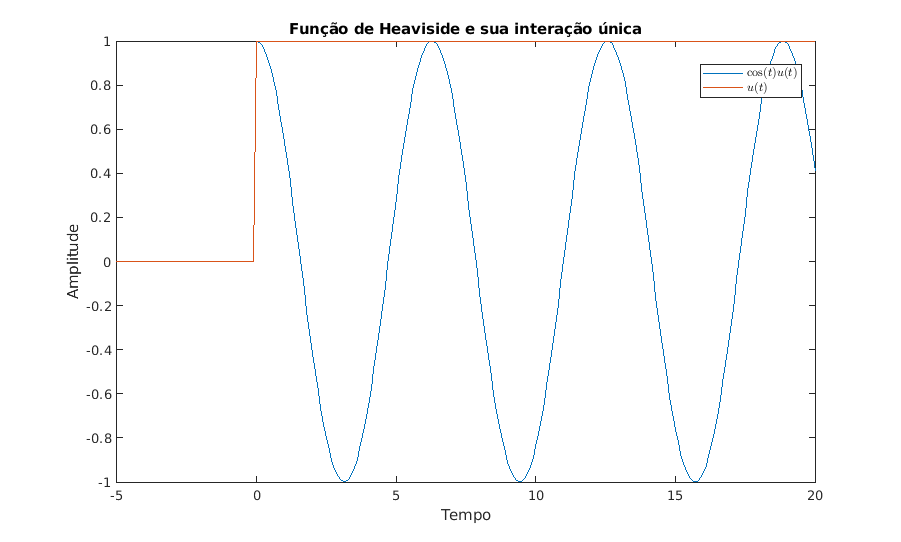
\includegraphics[width=\textwidth]{img/cos(t).png}
    \end{center}

    \subsubsection{Unidades de Medida}
    \begin{itemize}
        \item \textbf{Ohm [$\Omega$]}: resistência/impedância elétrica, relação entre a tensão e a corrente em um resistor.
        \item \textbf{Siemens [$S$]}: condutância/admitância elétrica, inverso da resistência. Esta unidade é também conhecida como \textbf{Mho [$\mho$]} ou \textbf{[$\Omega^{-1}$]}.
        \item \textbf{Henry [$H$]}: indutância elétrica, relação entre a tensão e a variação da corrente em um indutor.
        \item \textbf{Farad [$F$]}: capacitância, relação entre a carga elétrica e a tensão em um capacitor.
        \item \textbf{Watt [$W$]}: potência útil, calculada por $P=Vi$. Para indutores e capacitores existe a unidade \textbf{Volt-Ampère reativo [$VAr$]} que representa a potência reativa, e também deve ser citada a unidade \textbf{Volt-Ampère [$VA$]} que representa a potência aparente de um circuito de corrente alternada. As duas últimas não serão tratadas neste material
    \end{itemize}

    Além disso, existem alguns prefixos de unidades comuns na análise de circuitos elétricos.

    \begin{center}
        Relações dos prefixos das unidades \\
        \begin{tabular}{|c|c|c|} \hline
            Prefixo & Símbolo & Multiplicador \\ \hline
            Pico & $p$ & $10^{-12}$ \\
            Nano & $n$ & $10^{-9}$ \\
            Micro & $\mu$ & $10^{-6}$ \\
            Mili & $m$ & $10^{-3}$ \\
            Kilo & $k$ & $10^{3}$ \\
            Mega & $M$ & $10^{6}$ \\
            Giga & $G$ & $10^{9}$ \\ \hline
        \end{tabular}
    \end{center}

    \subsubsection{Teorema da Reciprocidade}
    Considerando um circuito elétrico resistivo com apenas uma fonte de corrente ou tensão, e um instrumento de medição voltímetro ou amperímetro, é possível permutar a fonte e o instrumento sem modificar a leitura do mesmo. Por exemplo

    \noindent\begin{minipage}{\textwidth}
    \begin{minipage}[b][5cm][b]{\dimexpr0.5\textwidth-0.5\Colsep\relax}
        \begin{center}
            \begin{circuitikz}[scale=0.95,transform shape]\draw
                (0,3) to[R,l=$R_1$] (0,0)
                (0,3) to[R,l=$R_2$] (3,3)
                (.5,3) -- (.5,4.5)
                (.5,4.5) to[voltmeter] (2.5,4.5)
                (2.5,4.5) -- (2.5,3)
                (3,3) to[V,l=$e_i$] (3,0)
                (3,3) to[R,l=$R_3$] (6,3)
                (6,3) to[R,l=$R_4$] (6,0)
                (0,0) -- (6,0)
            ;\end{circuitikz}
        \end{center}
    \end{minipage}
    \begin{minipage}[b][5cm][b]{\dimexpr0.5\textwidth-0.5\Colsep\relax}
        \begin{center}
            \begin{circuitikz}[scale=0.95,transform shape]\draw
                (0,3) to[R,l=$R_1$] (0,0)
                (0,3) to[R,l=$R_2$] (3,3)
                (.5,3) -- (.5,4.5)
                (.5,4.5) to[V,l=$e_i$] (2.5,4.5)
                (2.5,4.5) -- (2.5,3)
                (3,3) to[voltmeter] (3,0)
                (3,3) to[R,l=$R_3$] (6,3)
                (6,3) to[R,l=$R_4$] (6,0)
                (0,0) -- (6,0)
            ;\end{circuitikz}
        \end{center}
    \end{minipage}
    \end{minipage}

    \vspace{0.5cm}
    A tensão medida no voltímetro permanece a mesma nos dois casos. O Teorema de Reciprocidade extende-se também para fontes de corrente.

    \newpage

    \section{Circuitos Não Reativos}
    \label{sec:resistivos}

    \subsection{Operações básicas}

    \subsubsection{Divisor de Tensão}
    \label{subsubsec:divten}
    Em um circuito série contendo apenas uma fonte de tensão e resistores, pode-se expressar a tensão $V_{R_x}$ em um resistor $R_{x}$ por
    \begin{equation}
        V_{R_x}=\frac{R_{x}}{R_{eq}}V_{i}=\frac{R_{x}}{R_{x}+R_{a}}V_{i} \hspace{0.45cm}[V]
    \end{equation}
    Para indutores, a equação é análoga, portanto
    \begin{equation}
        V_{L_x}=\frac{L_{x}}{L_{eq}}V_{i}=\frac{L_{x}}{L_{x}+L_{a}}V_{i} \hspace{0.45cm}[V]
    \end{equation}
    Para capacitores, entretanto, a relação entre capacitância e tensão é de proporção inversa, portanto
    \begin{equation}
        V_{C_x}=\frac{C_{eq}}{C_{x}}V_{i}=\frac{C_{a}}{C_{x}+C_{a}}V_{i} \hspace{0.45cm}[V]
    \end{equation}

    \subsubsection{Divisor de Corrente}
    \label{subsubsec:divcor}
    Em um circuito paralelo contendo apenas uma fonte de corrente e resistores, pode-se expressar a corrente $i_{R_x}$ em um resistor $R_{x}$ por
    \begin{equation}
        i_{R_x}=\frac{R_{eq}}{R_{x}}i_{i}=\frac{R_{a}}{R_{x}+R_{a}}i_{i} \hspace{0.45cm}[A]
    \end{equation}
    Para indutores, a relação é análoga
    \begin{equation}
        i_{L_x}=\frac{L_{eq}}{L_{x}}i_{i}=\frac{L_{a}}{L_{x}+L_{a}}i_{i} \hspace{0.45cm}[A]
    \end{equation}
    Para capacitores, a corrente é diretamente proporcional à capacitância, portanto
    \begin{equation}
        i_{C_x}=\frac{C_{x}}{C_{eq}}i_{i}=\frac{C_{x}}{C_{x}+C_{a}}i_{i} \hspace{0.45cm}[A]
    \end{equation}

    \subsubsection{Thévenin}
    \label{subsubsec:thevenin}
    O Teorema de Thévenin (também chamado de Equivalente de Thévenin) é uma técnica de simplificação de circuitos que transforma uma rede de resistores e fontes(controladas ou não) em um circuito equivalente contendo uma fonte de tensão $V_{th}$ em série com um resistor $R_{th}$. Para tal, deve-se escolher dois terminais de interesse $a$ e $b$.

    Considerando uma rede genérica que contém apenas fontes independentes e resistores

    \begin{center}
        \begin{circuitikz}[scale=1.2,transform shape]\draw
            node[fourport](btt){}
            (btt.2) to[short,-*] ++(1,0) node[label={right:$b$}]{}
            (btt.3) to[short,-*] ++(1,0) node[label={right:$a$}]{}
        ;\end{circuitikz}
    \end{center}
    Por definição,
    \begin{itemize}
        \item $V_{th}$ é a tensão entre $a$ e $b$ a circuito aberto,
        \item $R_{th}$ é a resistência equivalente medida a partir dos terminais $a$ e $b$ após matar\footnote{Matar uma fonte é um termo informal para ``igualar o valor da fonte a zero''.} as fontes independentes (no caso de existirem fontes dependentes, deve-se utilizar o método descrito em seguida).
    \end{itemize}

    Deste modo, conseguimos simplificar a configuração do circuito elétrico, facilitando o cálculo de tensão e corrente em qualquer carga aplicada entre os terminais $a$ e $b$. Por exemplo, para encontrar o valor da tensão no capacitor $C$ pode-se aplicar o Teorema de Thévenin nos terminais indicados na figura

    \noindent\begin{minipage}{\textwidth}
    \begin{minipage}[c][4cm][c]{\dimexpr0.5\textwidth-0.5\Colsep\relax}
        \begin{center}
            \begin{circuitikz}[scale=0.9,transform shape]\draw
                (0,3) to[V,l=$e_i$] (0,0)
                (0,3) to[R,l=$R_1$] (3,3)
                (3,3) to[R,l=$R_2$] (3,0)
                (3,3) to[R,l=$R_3$] (6,3)
                (6,3) node[label={right:$a$}]{} to[C,l=$C$,v=$e_0$,*-*] (6,0) node[label={right:$b$}]{}
                (0,0) -- (6,0)
            ;\end{circuitikz}
        \end{center}
    \end{minipage}
    \begin{minipage}[c][4cm][c]{\dimexpr0.5\textwidth-0.5\Colsep\relax}
        Inicialmente, deve-se abrir o circuito nos terminais do capacitor ($a$ e $b$) e calcular a tensão que cai nos mesmos.
    \end{minipage}
    \end{minipage}

    \noindent\begin{minipage}{\textwidth}
    \begin{minipage}[c][4cm][c]{\dimexpr0.5\textwidth-0.5\Colsep\relax}
        \begin{center}
            \begin{circuitikz}[scale=0.9,transform shape]\draw
                (0,3) to[V,l=$e_i$] (0,0)
                (0,3) to[R,l=$R_1$] (3,3)
                (3,3) to[R,l=$R_2$,v=$V_{ab}$] (3,0)
                (3,3) to[R,l=$R_3$,v=$0V$,f=$0A$,-*] (6,3) node[label={right:$a$}]{}
                (0,0) to[short,-*] (6,0) node[label={right:$b$}]{}
            ;\end{circuitikz}
        \end{center}
    \end{minipage}
    \begin{minipage}[c][4cm][c]{\dimexpr0.5\textwidth-0.5\Colsep\relax}
        Como a tensão no resistor $R_3=0$, lembrando que um potencial é o mesmo ao longo de um fio ideal, a tensão $V_{ab}=V_{th}$ é exatamente a tensão que cai no resistor $R_2$, a qual pode ser calculado pelo divisor de tensão
        $$V_{th}=\frac{R_2}{R_1+R_2}e_i$$
    \end{minipage}
    \end{minipage}

    \noindent\begin{minipage}{\textwidth}
    \begin{minipage}[c][4cm][c]{\dimexpr0.5\textwidth-0.5\Colsep\relax}
        \begin{center}
            \begin{circuitikz}[scale=0.9,transform shape]\draw
                (0,3) to[short,*-*] (0,0)
                (0,3) to[R,l=$R_1$] (3,3)
                (3,3) to[R,l=$R_2$] (3,0)
                (3,3) to[R,l=$R_3$,v=$0V$,f=$0A$,-*] (6,3) node[label={right:$a$}]{}
                (0,0) to[short,-*] (6,0) node[label={right:$b$}]{}
            ;\end{circuitikz}
        \end{center}
    \end{minipage}
    \begin{minipage}[c][4cm][c]{\dimexpr0.5\textwidth-0.5\Colsep\relax}
        Em seguida, para o cálculo do resistor de Thévenin, mata-se a fonte de tensão (ou seja, deve-se substituí-la por um curto-circuito) e calcula-se a resistência equivalente vista dos terminais $a$ e $b$
    \end{minipage}
    \end{minipage}

    \noindent\begin{minipage}{\textwidth}
    \begin{minipage}[c][4cm][c]{\dimexpr0.5\textwidth-0.5\Colsep\relax}
        \begin{center}
            \begin{circuitikz}[scale=0.9,transform shape]\draw
                (0,3) to[R,l=$R_1$] (0,0)
                (0,3) -- (3,3)
                (3,3) to[R,l=$R_2$] (3,0)
                (3,3) to[R,l=$R_3$,-*] (6,3) node[label={right:$a$}]{}
                (0,0) to[short,-*] (6,0) node[label={right:$b$}]{}
            ;\end{circuitikz}
        \end{center}
    \end{minipage}
    \begin{minipage}[c][4cm][c]{\dimexpr0.5\textwidth-0.5\Colsep\relax}
        Rearranjando ligeiramente o $R_1$, percebe-se que o resistor equivalente é $R_3$ em série com o paralelo de $R_1$ e $R_2$, ou seja
        $$R_{th}=(R_1//R_2)+R_3=\frac{R_1R_2}{R_1+R_2}+R_3$$
    \end{minipage}
    \end{minipage}

    \noindent\begin{minipage}{\textwidth}
    \begin{minipage}[c][4cm][c]{\dimexpr0.5\textwidth-0.5\Colsep\relax}
        \begin{center}
            \begin{circuitikz}[scale=0.9,transform shape]\draw
                (0,3) to[V,l_=$\displaystyle\frac{R_2}{R_1+R_2}e_i$] (0,0)
                (0,3) to[R,l=$(R_1//R_2)+R_3$] (3,3) node[label={right:$a$}]{}
                (3,3) to[C,l=$C$,v=$e_0$,*-*] (3,0) node[label={right:$b$}]{}
                (0,0) -- (3,0)
            ;\end{circuitikz}
        \end{center}
    \end{minipage}
    \begin{minipage}[c][4cm][c]{\dimexpr0.5\textwidth-0.5\Colsep\relax}
        Deste modo, é possível escrever o circuito original como um circuito RC série (cuja solução será abordada em capítulos futuros), que torna simples encontrar a saída $e_0$.
    \end{minipage}
    \end{minipage}

    O interessante é que para qualquer combinação de componentes colocada entre os terminais, $a$ e $b$ terão o mesmo equivalente de Thévenin calculado, facilitando o cálculo para várias cargas diferentes.

    Outra técnica análoga é calcular o Equivalente de Norton, que transforma a rede de componentes em um circuito com uma fonte de corrente $I_{N}$ em paralelo com um resistor $I_{N}$. Neste caso,
    \begin{itemize}
        \item $I_{N}$ é a corrente de curto circuito de $a$ para $b$,
        \item $R_{N}$ é a resistência equivalente medida a partir dos terminais $a$ e $b$ após matar as fontes independentes (no caso de existirem fontes dependentes, deve-se utilizar o método descrito em seguida).
    \end{itemize}

    Tomando-se o mesmo exemplo,

    \noindent\begin{minipage}{\textwidth}
    \begin{minipage}[c][4cm][c]{\dimexpr0.5\textwidth-0.5\Colsep\relax}
        \begin{center}
            \begin{circuitikz}[scale=0.9,transform shape]\draw
                (0,3) to[V,l=$e_i$] (0,0)
                (0,3) to[R,l=$R_1$] (3,3)
                (3,3) to[R,l=$R_2$] (3,0)
                (3,3) to[R,l=$R_3$] (6,3)
                (6,3) node[label={right:$a$}]{} to[C,l=$C$,v=$e_0$,*-*] (6,0) node[label={right:$b$}]{}
                (0,0) -- (6,0)
            ;\end{circuitikz}
        \end{center}
    \end{minipage}
    \begin{minipage}[c][4cm][c]{\dimexpr0.5\textwidth-0.5\Colsep\relax}
        Deve-se trocar o capacitor por um curto-circuito e calcular a corrente que passa em $a-b$.
    \end{minipage}
    \end{minipage}

        \noindent\begin{minipage}{\textwidth}
        \begin{minipage}[c][4cm][c]{\dimexpr0.5\textwidth-0.5\Colsep\relax}
            \begin{center}
                \begin{circuitikz}[scale=0.9,transform shape]\draw
                    (0,3) to[V,l=$e_i$] (0,0)
                    (0,3) to[R,l=$R_1$] (3,3)
                    (3,3) to[R,l=$R_2$] (3,0)
                    (3,3) to[R,l=$R_3$] (6,3)
                    (6,3) to[short,f=$I_N$] (6,0)
                    (0,0) -- (6,0)
                ;\end{circuitikz}
            \end{center}
        \end{minipage}
        \begin{minipage}[c][4cm][c]{\dimexpr0.5\textwidth-0.5\Colsep\relax}
            Neste caso, para calcular a corrente $I_N$, pode-se associar $R_2$ e $R_3$ e em seguida dividir a tensão.
        \end{minipage}
        \end{minipage}

        \noindent\begin{minipage}{\textwidth}
        \begin{minipage}[c][4cm][c]{\dimexpr0.5\textwidth-0.5\Colsep\relax}
            \begin{center}
                \begin{circuitikz}[scale=0.9,transform shape]\draw
                    (0,3) to[V,l=$e_i$] (0,0)
                    (0,3) to[R,l=$R_1$] (3,3)
                    (3,3) to[R,l=$R_2//R_3$,v=V] (3,0)
                    (0,0) -- (3,0)
                ;\end{circuitikz}
            \end{center}
        \end{minipage}
        \begin{minipage}[c][4cm][c]{\dimexpr0.5\textwidth-0.5\Colsep\relax}
            $$V=\displaystyle\frac{\displaystyle\frac{R_2R_3}{R_2+R_3}}{R_1+\displaystyle\frac{R_2R_3}{R_2+R_3}}ei$$
            Como a tensão para componentes em paralelos é a mesma que cai em seu equivalente, temos que
            $$I_N=\frac{V}{R_3}=\displaystyle\frac{\displaystyle\frac{R_2}{R_2+R_3}}{R_1+\displaystyle\frac{R_2R_3}{R_2+R_3}}ei$$
        \end{minipage}
        \end{minipage}

        \noindent\begin{minipage}{\textwidth}
        \begin{minipage}[c][4cm][c]{\dimexpr0.5\textwidth-0.5\Colsep\relax}
            \begin{center}
                \begin{circuitikz}[scale=0.9,transform shape]\draw
                    (0,3) to[R,l=$R_1$] (0,0)
                    (0,3) -- (3,3)
                    (3,3) to[R,l=$R_2$] (3,0)
                    (3,3) to[R,l=$R_3$,-*] (6,3) node[label={right:$a$}]{}
                    (0,0) to[short,-*] (6,0) node[label={right:$b$}]{}
                ;\end{circuitikz}
            \end{center}
        \end{minipage}
        \begin{minipage}[c][4cm][c]{\dimexpr0.5\textwidth-0.5\Colsep\relax}
            Para o resistor $R_N$, percebe-se que o resistor equivalente é $R_3$ em série com o paralelo de $R_1$ e $R_2$, ou seja
            $$R_{th}=(R_1//R_2)+R_3=\frac{R_1R_2}{R_1+R_2}+R_3$$
        \end{minipage}
        \end{minipage}

        \noindent\begin{minipage}{\textwidth}
        \begin{minipage}[c][4cm][c]{\dimexpr0.7\textwidth-0.5\Colsep\relax}
            \begin{center}
                \begin{circuitikz}[scale=0.9,transform shape]\draw
                    (0,0) to[I,l=$\displaystyle\frac{\displaystyle\frac{R_2}{R_2+R_3}}{R_1+\displaystyle\frac{R_2R_3}{R_2+R_3}}ei$] (0,3)
                    (0,3) -- (3.5,3)
                    (3.5,3) to[R,l_=$(R_1//R_2)+R_3$] (3.5,0)
                    (3.5,3) -- (6,3)
                    (6,3) node[label={right:$a$}]{} to[C,l=$C$,v=$e_0$,*-*] (6,0) node[label={right:$b$}]{}
                    (0,0) -- (6,0)
                ;\end{circuitikz}
            \end{center}
        \end{minipage}
        \begin{minipage}[c][4cm][c]{\dimexpr0.3\textwidth-0.5\Colsep\relax}
            O circuito se limita a um RC em paralelo.
        \end{minipage}
        \end{minipage}


    É possível transformar um equivalente Thévenin em um equivalente Norton e vice-versa escolhendo os terminais $a$ e $b$ da seguinte maneira

    \noindent\begin{minipage}{\textwidth}
    \begin{minipage}[c][4cm][c]{\dimexpr0.45\textwidth-0.5\Colsep\relax}
        \begin{center}
            \begin{circuitikz}[scale=0.9,transform shape]\draw
                (0,0) to[I,l=$I_N$] (0,3)
                (0,3) to[short,-*] (4,3) node[label={right:$a$}]{}
                (3,3) to[R,l_=$R_N$] (3,0)
                (0,0) to[short,-*] (4,0) node[label={right:$b$}]{}
            ;\end{circuitikz}
        \end{center}
    \end{minipage}
    \begin{minipage}[c][4cm][c]{\dimexpr0.1\textwidth-0.5\Colsep\relax}
        $\iff$
    \end{minipage}
    \begin{minipage}[c][4cm][c]{\dimexpr0.45\textwidth-0.5\Colsep\relax}
        \begin{circuitikz}[scale=0.9,transform shape]\draw
            (0,3) to[V,l_=$E_{th}$] (0,0)
            (0,3) to[R,l=$R_{th}$,-*] (3,3) node[label={right:$a$}]{}
            (0,0) to[short, -*] (3,0) node[label={right:$b$}]{}
        ;\end{circuitikz}
    \end{minipage}
    \end{minipage}

    Utilizando as relações da Lei de Ohm
    $$ R_{th}=R_{N} $$
    \begin{equation}
        E_{th}=R_{N}I_{N}
    \end{equation}
    \begin{equation}
        I_{N}=\frac{E_{th}}{R_{th}}
    \end{equation}

    \subsubsection{Equivalente Thévenin/Norton com fontes controladas}
    \label{subsubsec:thfontecontrolada}
    Apesar de a maneira de calcular $V_{th}$ e $I_N$ seja a mesma, não é possível calcular $R_{th}$ e $R_N$ por associação. Por isso, deve-se utilizar uma outra maneira (que é sempre válida, porém um pouco mais trabalhosa). O método consiste em aplicar uma fonte com um valor conhecido e utilizar a Lei de Ohm para obter o valor do resistor. A mais clássica escolha é calcular a tensão que cai nos terminais de uma fonte de corrente de $1A$. Já que $V=Ri$, para $i=1A$, $V=R$. Do mesmo exemplo, tem-se

    \noindent\begin{minipage}{\textwidth}
    \begin{minipage}[c][4cm][c]{\dimexpr0.5\textwidth-0.5\Colsep\relax}
        \begin{center}
            \begin{circuitikz}[scale=0.9,transform shape]\draw
                (0,3) -- (0,0)
                (0,3) to[R,l=$R_1$] (3,3)
                (3,3) to[R,l=$R_2$] (3,0)
                (3,3) to[R,l=$R_3$,-*] (6,3) node[label={right:$a$}]{}
                (0,0) to[short,-*] (6,0) node[label={right:$b$}]{}
                (6,0) to[I,l_=$1A$,v^=$R_{th}$] (6,3)
            ;\end{circuitikz}
        \end{center}
    \end{minipage}
    \begin{minipage}[c][4cm][c]{\dimexpr0.5\textwidth-0.5\Colsep\relax}
        Neste caso a tensão que cai na fonte é
        $$R_{th}=[(R_1//R_2)+R_3]\hspace{0.05cm} 1A$$
        Que é o exato mesmo valor encontrado nos outros casos
    \end{minipage}
    \end{minipage}

    Tomando-se um novo exemplo, com uma fonte controlada de corrente

    \noindent\begin{minipage}{\textwidth}
    \begin{minipage}[c][4cm][c]{\dimexpr0.45\textwidth-0.5\Colsep\relax}
        \begin{center}
            \begin{circuitikz}[scale=0.88,transform shape]\draw
                (0,3) to[V,l=$10V$] (0,0)
                (0,3) to[R,l=$1\Omega$,v=$v$] (3,3)
                (3,0) to[I,l=$3v$] (3,3)
                (3,3) to[R,l=$1\Omega$] (6,3)
                (6,3) node[label={right:$a$}]{} to[C,l=$C$,v=$e_0$,*-*] (6,0) node[label={right:$b$}]{}
                (0,0) -- (6,0)
            ;\end{circuitikz}
        \end{center}
    \end{minipage}
    \begin{minipage}[c][4cm][c]{\dimexpr0.1\textwidth-0.5\Colsep\relax}
        $\implies$
    \end{minipage}
    \begin{minipage}[c][4cm][c]{\dimexpr0.45\textwidth-0.5\Colsep\relax}
        \begin{center}
            \begin{circuitikz}[scale=0.88,transform shape]\draw
                (0,3) -- (0,0)
                (0,3) to[R,l=$1\Omega$,v=$v$] (3,3)
                (3,0) to[I,l=$3v$] (3,3)
                (3,3) to[R,l=$1\Omega$] (6,3)
                (6,0) node[label={right:$b$}]{} to[I,l_=$1A$,v^=$R_{th}$,*-*] (6,3) node[label={right:$a$}]{}
                (0,0) -- (6,0)
            ;\end{circuitikz}
        \end{center}
    \end{minipage}
    \end{minipage}

    \noindent\begin{minipage}{\textwidth}
    \begin{minipage}[c][5cm][c]{\dimexpr0.5\textwidth-0.5\Colsep\relax}
        \begin{center}
            \begin{circuitikz}[scale=0.9,transform shape]\draw
                (0,3) -- (0,0)
                (0,3) to[R,l=$1\Omega$,v=$v$,f=$v$] (3,3)
                (3,0) to[I,l=$3v$] (3,3)
                (3,3) to[R,l=$1\Omega$,v<=$1V$,f<=$1A$] (6,3)
                (6,0) node[label={right:$b$}]{} to[I,l_=$1A$,v^=$R_{th}$,*-*] (6,3) node[label={right:$a$}]{}
                (0,0) -- (6,0)
            ;\end{circuitikz}
        \end{center}
    \end{minipage}
    \begin{minipage}[c][5cm][c]{\dimexpr0.5\textwidth-0.5\Colsep\relax}
        Através da equação de nó do circuito, têm-se que
        $$v+3v+1=0$$
        Ou seja,
        $$v=-\frac{1}{4}=-0.25V$$
        Então, pode-se calcular $R_{th}$ utilizando a malha que envolve ambos os resistores e a fonte de $1A$
        $$R_{th}=1-v=1.25\Omega$$
    \end{minipage}
    \end{minipage}

    \textbf{Observação:} Formalmente, a definição do resistor de Thévenin é a razão entre a tensão a circuito aberto e a corrente de curto-circuito. Entretanto, os autores julgam os métodos aqui apresentados mais eficientes, visto que envolvem a resolução de apenas um circuito, ao invés de dois (um com os terminais abertos e outro com os terminais fechados).

    \subsubsection{Transformação de Fonte}
    \label{subsubsec:transform}
    A transformação de fonte consiste em encontrar o equivalente de Thévenin/Norton de uma fonte e um resistor associados. Existem quatro combinações entre resistor em série ou paralelo e fonte de tensão ou corrente. Nos casos de uma fonte de tensão em paralelo com um resistor ou de uma fonte de corrente em série com um resistor, o equivalente é exatamente o mesmo circuito (ou seja, não é útil transformar). Convém, então, analisar apenas os outros dois casos.
    \begin{itemize}
        \item Fonte de tensão em série com um resistor:
            \begin{center}
                \begin{circuitikz}\draw
                    (0,2) to[V,l=$V$] (0,0)
                    (0,2) to[R,l=$R$,-*] (2,2) node[label={right:$a$}]{}
                    (0,0) to[short, -*] (2,0) node[label={right:$b$}]{}
                ;\end{circuitikz}
            \end{center}

            Naturalmente, a corrente de curto circuito é $i_{N}=\displaystyle\frac{V}{R}$ e a resistência de Norton é o próprio resistor $R_{N}=R$

            Então, uma fonte de tensão $V$ em série com um resistor $R$ é equivalente a uma fonte de corrente $\displaystyle\frac{V}{R}$ em paralelo com um resistor $R$
        \item Fonte de corrente em paralelo com um resistor:
            \begin{center}
                \begin{circuitikz}\draw
                    (0,0) to[I,l=$I$] (0,2)
                    (2,2) to[R,l=$R$] (2,0)
                    (0,2) to[short, -*] (3,2) node[label={right:$a$}]{}
                    (0,0) to[short, -*] (3,0) node[label={right:$b$}]{}
                ;\end{circuitikz}
            \end{center}
            A tensão a circuito aberto é $V_{th}=RI$ e a resistência equivalente é o próprio resistor $R_{th}=R$

            Logo, uma fonte de corrente $I$ em paralelo com um resistor $R$ é equivalente a uma fonte de tensão $RI$ em série com um resistor $R$
    \end{itemize}

    Nota-se que as transformações são reversíveis, posto que é possível transformar novamente o circuito já transformado.

    \noindent\begin{minipage}{\textwidth}
    \begin{minipage}[c][4cm][c]{\dimexpr0.45\textwidth-0.5\Colsep\relax}
        \begin{center}
            \begin{circuitikz}\draw
                (0,0) to[I,l=$I$] (0,2)
                (2,2) to[R,l=$R$] (2,0)
                (0,2) to[short, -*] (3,2) node[label={right:$a$}]{}
                (0,0) to[short, -*] (3,0) node[label={right:$b$}]{}
            ;\end{circuitikz}
        \end{center}
    \end{minipage} \hfill
    \begin{minipage}[c][4cm][c]{\dimexpr0.1\textwidth-0.5\Colsep\relax}
        $$\iff$$
    \end{minipage} \hfill
    \begin{minipage}[c][4cm][c]{\dimexpr0.45\textwidth-0.5\Colsep\relax}
        \begin{center}
            \begin{circuitikz}\draw
                (0,2) to[V,l=$RI$] (0,0)
                (0,2) to[R,l=$R$,-*] (2,2) node[label={right:$a$}]{}
                (0,0) to[short, -*] (2,0) node[label={right:$b$}]{}
            ;\end{circuitikz}
        \end{center}
    \end{minipage}
    \end{minipage}

    \subsubsection{Explosão de Fonte}
    \label{subsubsec:explosion}
    Explosão de fonte é uma técnica que permite ``deslocar'' uma fonte sem alterar a sua contribuição para com o circuito elétrico. À rigor, apenas reescreve-se o circuito de modo que facilite a resolução. Esta técnica é muitas vezes utilizada juntamente com as transformações para a simplificação de malhas.
    \begin{itemize}
        \item \textbf{Fonte de tensão:} Uma fonte de tensão pode ser ``explodida'' em um nó, desde que os mesmos potenciais estejam associados às mesmas cargas.

        \begin{center}
        \noindent\begin{minipage}{0.8\textwidth}
        \begin{minipage}[c][4cm][c]{\dimexpr0.45\textwidth-0.5\Colsep\relax}
            \begin{center}
                \begin{circuitikz}[scale=0.9,transform shape]\draw
                    (0,2) to[V,l=$V$] (0,0)
                    (0,2) to[short,-*] (2,2) node[label={above:$b$}]{}
                    (0,2) -- (0,4)
                    (0,4) to[short,-*] (2,4) node[label={above:$a$}]{}
                    (0,0) to[short,-*] (2,0) node[label={above:$c$}]{}
                    (2,0) -- (4,0)
                    (2,2) to[R,l=$R_b$] (4,2)
                    (2,4) to[R,l=$R_a$] (4,4)
                    (4,0) -- (4,4)
                ;\end{circuitikz}
            \end{center}
        \end{minipage} \hfill
        \begin{minipage}[c][4cm][c]{\dimexpr0.1\textwidth-0.5\Colsep\relax}
            $$\iff$$
        \end{minipage} \hfill
        \begin{minipage}[c][4cm][c]{\dimexpr0.45\textwidth-0.5\Colsep\relax}
            \begin{center}
                \begin{circuitikz}[scale=0.9,transform shape]\draw
                    (0,2) -- (0,0)
                    (2,2) node[label={above:$b$}]{} to[V,l=$V$,*-] (0,2)
                    (0,2) -- (0,4)
                    (2,4) node[label={above:$a$}]{} to[V,l=$V$,*-] (0,4)
                    (0,0) to[short,-*] (2,0) node[label={above:$c$}]{}
                    (2,0) -- (4,0)
                    (2,2) to[R,l=$R_b$] (4,2)
                    (2,4) to[R,l=$R_a$] (4,4)
                    (4,0) -- (4,4)
                ;\end{circuitikz}
            \end{center}
        \end{minipage}
        \end{minipage}
        \end{center}

        Nota-se em ambos os circuitos que os pontos $a$ e $b$ ``enxergam'' o potencial positivo de $V$ e que $c$ ``enxerga'' o potencial negativo de $V$. Todas as tensões e correntes são exatamente as mesmas, portanto, os circuitos são equivalentes.

        \item \textbf{Fonte de corrente:} Uma fonte de corrente pode ser ``explodida'' em uma malha, desde que as mesmas correntes entrem e saiam de todos os nós.

        \noindent\begin{minipage}{0.8\textwidth}
        \begin{minipage}[c][5cm][c]{\dimexpr0.45\textwidth-0.5\Colsep\relax}
            \begin{center}
                \begin{circuitikz}[scale=0.9,transform shape]\draw
                    (0,0) to[I,l=$I$] (4,0)
                    (0,2) to[R,l=$R_a$,-*] (2,2) node[label={above:$a$}]{}
                    (2,2) to[R,l=$R_b$,-*] (4,2)
                    (4,0) -- (4,2)
                    (0,0) -- (0,2)
                ;\end{circuitikz}
            \end{center}
        \end{minipage} \hfill
        \begin{minipage}[c][5cm][c]{\dimexpr0.1\textwidth-0.5\Colsep\relax}
            $$\iff$$
        \end{minipage} \hfill
        \begin{minipage}[c][5cm][c]{\dimexpr0.45\textwidth-0.5\Colsep\relax}
            \begin{center}
                \begin{circuitikz}[scale=0.9,transform shape]\draw
                    (0,0) to[I,l=$I$] (2,0)
                    (2,0) to[I,l=$I$] (4,0)
                    (2,0) to[short,f=$0$] (2,2)
                    (0,2) to[R,l=$R_a$,-*] (2,2) node[label={above:$a$}]{}
                    (2,2) to[R,l=$R_b$] (4,2)
                    (4,0) -- (4,2)
                    (0,0) -- (0,2)
                ;\end{circuitikz}
            \end{center}
        \end{minipage}
        \end{minipage}

        Na segunda figura, percebe-se que foram adicionadas duas fontes de corrente $I$, arranjadas de modo que os valores das correntes em ambos circuitos são os mesmos. Portanto, é um equivalente válido.
    \end{itemize}

    Por exemplo, considere o circuito abaixo, dados $R_1=20 \Omega$, $R_2=125 \Omega$, $R_0=400 \Omega$, $C=1 mF$, $\mu = 0.01 \frac{A}{V}$, $e_i=5 u(t)$.

    \noindent\begin{minipage}{0.95\textwidth}
    \begin{minipage}[c][7cm][c]{\dimexpr0.6\textwidth-0.5\Colsep\relax}
        \begin{center}
            \begin{circuitikz}[scale=0.9,transform shape]\draw
                (0,4) to[V=$e_i$] (0,0)
                (0,4) to[short,-*] (2,4)
                (2,4) to[open,v=$v$] (2,2)
                (2,2) to[short,*-] (3,2)
                (3,2) to[R,l=$R_1$] (3,0)
                (3,2) -- (4,2)
                (4,4) to[I,l_=$\mu v$] (4,2)
                (4,4) -- (6,4)
                (6,4) to[R,l=$R_0$] (6,2)
                (4,2) -- (6,2)
                (6,4) -- (8,4)
                (8,4) to[R,l=$R_2$,v=$e_0$] (8,0)
                (0,0) -- (8,0)
                (0,4) -- (0,6)
                (0,6) to[C,l=$C$] (8,6)
                (8,6) -- (8,4)
            ;\end{circuitikz}
        \end{center}
    \end{minipage} \hfill
    \begin{minipage}[c][7cm][c]{\dimexpr0.4\textwidth-0.5\Colsep\relax}
        Inicialmente, este circuito pode parecer complexo, porém, pode-se utilizar explosão de fonte em $e_i$, de modo que
    \end{minipage}
    \end{minipage}

    \noindent\begin{minipage}{0.95\textwidth}
    \hspace{0.01cm}
    \begin{minipage}[c][7cm][c]{\dimexpr0.6\textwidth-0.5\Colsep\relax}
        \begin{center}
            \begin{circuitikz}[scale=0.9,transform shape]\draw
                (0,4) -- (0,0)
                (2,4) to[V,l=$e_i$,*-] (0,4)
                (2,4) to[open,v=$v$] (2,2)
                (2,2) to[short,*-] (3,2)
                (3,2) to[R,l=$R_1$] (3,0)
                (3,2) -- (4,2)
                (4,4) to[I,l_=$\mu v$] (4,2)
                (4,4) -- (6,4)
                (6,4) to[R,l=$R_0$] (6,2)
                (4,2) -- (6,2)
                (6,4) -- (8,4)
                (8,4) to[R,l=$R_2$,v=$e_0$] (8,0)
                (0,0) -- (8,0)
                (0,4) -- (0,6)
                (2,6) to[V,l=$e_i$] (0,6)
                (2,6) to[C,l=$C$] (8,6)
                (8,6) -- (8,4)
            ;\end{circuitikz}
        \end{center}
    \end{minipage} \hfill
    \begin{minipage}[c][7cm][c]{\dimexpr0.4\textwidth-0.5\Colsep\relax}
        Analisando os potenciais do circuito, percebe-se que o ramo do capacitor está em paralelo com o ramo do resistor $R_2$ ($e_i$ em um terminal e $0$ em outro), o que permite rearranjar o circuito sem afetar os valores de tensão e corrente no mesmo.
    \end{minipage}
    \end{minipage}

    \begin{center}
        \begin{circuitikz}[scale=0.9,transform shape]\draw
            (0,4) -- (0,0)
            (2,4) to[V,l=$e_i$,*-] (0,4)
            (2,4) to[open,v=$v$] (2,2)
            (2,2) to[short,*-] (3,2)
            (3,2) to[R,l=$R_1$] (3,0)
            (3,2) -- (4,2)
            (4,4) to[I,l_=$\mu v$] (4,2)
            (4,4) -- (6,4)
            (6,4) to[R,l=$R_0$] (6,2)
            (4,2) -- (6,2)
            (6,4) to[short,-*] (7,4) node[label={above:$a$}]{}
            (7,4) -- (8,4)
            (8,4) to[R,l=$R_2$,v=$e_0$] (8,0)
            (0,0) to[short,-*] (7,0) node[label={above:$b$}]{}
            (7,0) -- (10,0)
            (10,4) -- (8,4)
            (10,2) to[V,l=$e_i$] (10,0)
            (10,4) to[C,l=$C$] (10,2)
        ;\end{circuitikz}
    \end{center}

    Com o circuito escrito neste formato, pode-se calcular o equivalente de Thévenin em relação aos terminais $a$ e $b$

    \begin{center}
        \begin{circuitikz}\draw
            (0,4) to[V,l=$e_i$] (0,0)
            (2,4) to[short,*-] (0,4)
            (2,4) to[open,v=$v$] (2,2)
            (2,2) to[short,*-] (3,2)
            (3,2) to[R,l=$R_1$,v=$0V$] (3,0)
            (3,2) to[short,f<=$0A$] (4,2)
            (4,4) to[I,l_=$\mu v$,-*] (4,2) node[label={below:$2$}]{}
            (4,4) -- (6,4)
            (6,4) to[R,l=$R_0$,v<=$\mu R_0v$] (6,2)
            (4,2) to[short,f_=$\mu v$] (6,2)
            (6,4) to[short,f=$0A$,-*] (8,4) node[label={right:$a$}]{}
            (0,0) to[short,f_<=$0A$,-*] (3,0) node[label={below:$1$}]{}
            (3,0) to[short,f_=$0A$] (7,0)
            (7,0) to[short,-*] (8,0) node[label={right:$b$}]{}
            (7.9,4) to[open,v=$E_{th}$] (7.9,0)
        ;\end{circuitikz}
    \end{center}

    Já que a corrente em um circuito aberto é igual a $0A$, utilizando o nó $1$, descobre-se que a corrente no resistor $R_1$ é, também, igual a $0A$, o que implica tensão $0V$ no mesmo. Através da análise do nó $2$, percebe-se que a corrente da fonte controlada de corrente vai toda para o resistor $R_0$, polarizando-o como mostrado.
    A partir daí, pode-se calcular $E_{th}$ pela malha que contém $R_0$ e $R_1$, ou seja

    $$E_{th}=-\mu R_0v$$

    Porém, devemos relacionar a tensão $v$ do elemento controlado com a entrada $e_i$, para manter nosso equivalente diretamente relacionado com a mesma. Isso é alcançável utilizando a malha que contém $e_i$, $v$ e $R_0$

    $$e_i=v+0$$

    Ou seja,

    $$E_{th}=-\mu R_0e_i$$
    $$E_{th}=-20V$$

    Então, para calcular o resistor $R_{th}$, aplica-se uma fonte de $1A$ entre os terminais $a$ e $b$ e mata-se as fontes independentes.

    \begin{center}
        \begin{circuitikz}\draw
            (0,4) -- (0,0)
            (2,4) to[short,*-] (0,4)
            (2,4) to[open,v=$v$] (2,2)
            (2,2) to[short,*-] (3,2)
            (3,2) to[R,l=$R_1$,v=$R_1$] (3,0)
            (3,2) to[short] (4,2)
            (4,4) to[I,l_=$\mu v$,-*] (4,2) node[label={below:$2$}]{}
            (4,4) -- (6,4)
            (6,4) to[R,l=$R_0$,v<=$ $] (6,2)
            (4,2) to[short,f_=$\mu v - 1$] (6,2)
            (6,4) to[short,-*] (8,4) node[label={right:$a$}]{}
            (0,0) to[short,f_<=$0A$,-*] (3,0) node[label={below:$1$}]{}
            (3,0) to[short] (7,0)
            (7,0) to[short,-*] (8,0) node[label={right:$b$}]{}
            (8,0) to[I,l=$1A$,v=$R_{th}$] (8,4)
        ;\end{circuitikz}
    \end{center}

    Neste caso, a corrente em $R_1$ é $1A$, portanto sua tensão é $R_1$, o que resulta, pela malha à esquerda, na relação

    $$v=-R_1$$

    Além disso, pelo nó $2$, a corrente no resistor $R_0$, polarizada conforme a imagem, deve ser $i_{R_0}=\mu v - 1$, portanto, equacionando a malha à direita,

    $$R_{th}=R_1-R_0[\mu v-1]=R_1-R_0[-\mu R_1-1]$$
    $$R_{th}=R_1+R_0+\mu R_0R_1$$
    $$R_{th}=500 \Omega$$

    Portanto, o circuito equivalente é

    \begin{center}
        \begin{circuitikz}\draw
            (0,2) to[V,l_=$V_{th}$] (0,0)
            (0,2) to[R,l=$R_{th}$] (2,2)
            (2,2) to[R,l=$R_2$,v=$e_0$] (2,0)
            (2,2) -- (4,2)
            (4,2) to[C,l=$C$] (4,0)
            (0,0) -- (4,0)
        ;\end{circuitikz}
    \end{center}

    Que é muito mais simples em comparação ao circuito original. O método de resolução de circuitos capacitivos será abordado em capítulos futuros.

    \subsubsection{Balanço de Potência}
    \label{subsubsec:balancodepot}
    A partir do conceito da conservação de energia, é possível equacionar a potência dos componentes de um circuito elétrico através da relação
    \begin{equation}
        \sum_{k=1}^{n} \displaystyle{P_{k_{dissipada}}}=\displaystyle{\sum_{k=1}^{m} P_{k_{fornecida}}} \hspace{0.25cm} ,
    \end{equation}

    \noindent o que nos permite fazer o balanço de potências, ou seja, calcular as potências individuais de cada componente e somá-las. Este tipo de técnica é muito útil para checar exercícios, posto que no caso em que a potência dissipada é igual à fornecida a energia foi conservada. As definições de potência dissipada e fornecida seguem a convenção
    \begin{itemize}
        \item \hspace{0.2cm} A potência é dissipada quando as cargas elétricas passam de um ponto de \textbf{maior} potencial elétrico para um de \textbf{menor} potencial elétrico. Em outras palavras, quando a corrente corre do terminal polarizado positivamente $(+)$ para o polarizado negativamente $(-)$. Pode-se dizer que o componente ``consumiu'' potência do sistema.
        \item \hspace{0.2cm} A potência é fornecida quando as cargas elétricas passam do ponto com \textbf{menor} potencial elétrico $(-)$ para um de \textbf{maior} potencial elétrico $(+)$. Pode-se dizer que o elemento é ``fonte'' de potência elétrica para o sistema.
    \end{itemize}

    \subsection{Diodos}
    \label{subsec:diodos}
    Um diodo é um elemento não-linear composto por semicondutores (geralmente cristais de silício ou germânio) polarizados em duas regiões, uma do tipo N e outra do tipo P, que, na maioria das vezes, permite fácil passagem de corrente em polarização direta e dificulta a passagem de corrente em polarização reversa. Existem diversos modelos de diodos, desde o ideal (mais simples, porém pouco prático em aplicações) até o diodo real (maior nível de complexidade, porém útil em casos que requerem alta precisão). Este material contém apenas o modelo ideal de um diodo.

    \subsubsection{Diodos Ideais}
    \label{subsubsec:diodos}
    Os diodos ideais funcionam exclusivamente como elemento de chaveamento. Assume-se que, em condução, o diodo possui queda de tensão $V_{D}=0 \hspace{0.2cm}[V]$, ou seja, é um curto circuito. Em polarização reversa, entretanto, o diodo ideal se comporta como uma impedância infinita, impossibilitando a passagem de corrente entre seus terminais.
    \begin{center}
        \begin{circuitikz}\draw
            (0,0) to[D,v=$V$,f=$i$,*-*] (3,0)
        ;\end{circuitikz}
    \end{center}

    Se o efeito de $V$ polarizar o diodo diretamente ($V>0$), diz-se que o diodo está no modo \textbf{ON} e têm-se $i>0$. Neste caso, ao constatar que o diodo está conduzindo, pode-se substituí-lo por um curto circuito, visto que ele permitirá a passagem da corrente sem alterar a tensão do circuito. Do contrário, o diodo está \textbf{OFF} e seu modelo é um circuito aberto.

    \subsection{Amplificador Operacional Ideal}
    \label{subsec:ampop}
    Um amplificador operacional (AmpOp) é um componente que tem como saída um sinal de entrada amplificado. No caso ideal, considera-se o ganho $G=\displaystyle{\frac{V_{o}}{V_{i}}}$ infinito. Este componente possui dois terminais de entrada, as portas inversora $(-)$ e não-inversora $(+)$ e um terminal de saída, além de dois terminais de alimentação $(+V_{CC}$ e $-V_{CC})$. Idealmente o AmpOp possui uma impedância de entrada infinita, bem como uma impedância de saída zero, ou seja, um sinal de tensão é perfeitamente amplificado para a saída, sem nenhum tipo de perda. \\
    %Imagem do AmpOp%
    *INSERT IMAGE*

    É evidente que no mundo real não é possível obter ganho infinito ou impedâncias infinitas ou zero. O que realmente acontece é que, a partir de um certo ponto, a tensão de saída do amplificador operacional é saturada de acordo com as tensões de alimentação. A impedância de entrada é muito alta e a impedância de saída é muito baixa. \\
    Os amplificadores operacionais possuem diversas aplicações, sendo a mais básica delas um comparador de tensão (o maior valor entre $V_{+}$ e $V_{-}$ será amplificado, saturando a saída em $+V_{CC}$ ou $-V_{CC})$. Em grande parte das aplicações, utiliza-se de uma configuração em \textbf{malha fechada}, quando o circuito é realimentado (feedback). As aplicações a seguir utilizam a realimentação negativa, ou seja, a saída do AmpOp é conectada à entrada inversora através de uma rede de componentes.\\
    %AmpOp realimentação negativa%
    *INSERT IMAGE*
    Esta ligação tem como característica a criação do chamado \textbf{curto-circuito virtual} entre seus terminais. Em outras palavras, a tensão entre as entradas inversora e não-inversora é igual a zero. Lembrando que, como a impedância de entrada é muito alta, considera-se a corrente de entrada igual a zero. \\
    %AmpOp mostrando curto virtual e corrente de entrada zero%
    *INSERT IMAGE*
    \subsubsection{Configuração Inversora}
    A aplicação de tensão na porta inversora causa um ganho na saída proporcional e com sinal oposto ao da entrada. No caso geral
    %AmpOp inversor com Ri e Rf%
    *INSERT IMAGE*
    \begin{equation}
        G=\frac{V_{o}}{V_{i}}=-\frac{R_{f}}{R_{i}}
    \end{equation}
    \subsubsection{Configuração Não-Inversora}
    A aplicação de tensão na porta não-inversora causa um ganho proporcional à entrada, sem mudança de sinal. \\
    %AmpOp Não-inversor com Ri e Rf%
    *INSERT IMAGE*
    \begin{equation}
        G=\frac{V_{o}}{V_{i}}=1+\frac{R_{f}}{R_{i}}
    \end{equation}

    \subsubsection{Configuração Seguidor de Tensão}
    Caso particular do amplificador não-inversor em que as resistências $R_{i}$ e $R_{f}$ são iguais a, respectivamente, infinito e $0$ (caso ideal), fazendo com que o ganho seja unitário, o que implica a tensão de saída ser igual à de entrada.
    %AmpOp não-inversor sem resistências.
    *INSERT IMAGE*
    \begin{equation}
        G=\frac{V_{o}}{V_{i}}=1+\frac{R_{f}}{R_{i}}=1+\frac{0}{\infty}\xrightarrow{}1
    \end{equation}

    \subsubsection{Configuração Somador de Tensão}
    A aplicação de $n$ fontes de tensão gera uma ganho inverso à soma ponderada das entradas.
    %AmpOp somador inversor com n entradas%
    *INSERT IMAGE*
    \begin{equation}
        G=\frac{V_{o}}{V_{i}}=-(\frac{R_{f}}{R_{1}}V_{1}+\frac{R_{f}}{R_{2}}V_{2}+...+\frac{R_{f}}{R_{n}}V_{n})=-\sum_{k=1}^{n}\frac{R_{f}}{R_{k}}V_{k}
    \end{equation}

    \subsubsection{Configuração Amplificador de Diferenças}
    Trabalha como amplificador da tensão diferencial $V_{d}=V_{+}-V_{-}$ entre os terminais de entrada. %AmpOp amplificador de diferenças com R1(-),R2(feedback),R3(+),R4(ground), fontes V2+ e V1-%
    *INSERT IMAGE*

    Usando o teorema da superposição,
    \begin{equation*}
        V_{o}=\frac{1+\displaystyle\frac{R_{2}}{R_{1}}}{1+\displaystyle\frac{R_{3}}{R_{4}}}V_{2} - \displaystyle\frac{R_{2}}{R_{1}}V_{1}
    \end{equation*}
    No caso particular em que $R_{1}=R_{3}$ e $R_{2}=R_{4}$
    \begin{equation}
        V_{o}=\frac{R_{2}}{R_{1}}V_{2}-\frac{R_{2}}{R_{1}}V_{1}=\frac{R_{2}}{R_{1}}V_{d}
    \end{equation}

    \subsection{Quadripolos}
    \label{subsec:quadripolos}
    Quadripolo é o nome dado a uma rede de componentes que se liga com algum outro circuito por apenas dois pares de terminais. São definidas as tensão nas portas $V_{1}$ e $V_{2}$ polarizadas simetricamente e as correntes nas portas $I_{1}$ e $I_{2}$ entrando no quadripolo. \\
    %Quadripolo genérico com V1,I1, V2,I2%
    *INSERT IMAGE*

    A relação entre as tensões e correntes varia de acordo com o tipo de \textbf{parâmetro} escolhido durante a sua modelagem. Este tipo de componente é muito útil na simplificação de circuitos com muitos elementos, já que, uma vez obtidos os parâmetros, relaciona as tensões e correntes sem precisar saber o conteúdo do quadripolo.

    \subsubsection{Parâmetros r}
    \label{subsubsec:quadripolosr}
    Os parâmetros resistivos ($r$) ou impedância ($z$) relacionam as tensões $V_{1}$ e $V_{2}$ como uma combinação linear das correntes $I_{1}$ e $I_{2}$, ou seja
    \begin{equation*}
        V_{1}=r_{11}I_{1}+r_{12}I_{2}
    \end{equation*}
    \begin{equation*}
        V_{2}=r_{21}I_{1}+r_{22}I_{2}
    \end{equation*}
    Essas equações podem ser reescritas na forma matricial, de modo que

    \begin{equation*}
        \textbf{V}=\text{R}\textbf{I}, \hspace{0.3cm} \text{ou}
    \end{equation*}

    \begin{equation}
        %Matriz V
        \begin{bmatrix}
            V_{1} \\
            V_{2}
        \end{bmatrix}
        = %Matriz R
        \begin{bmatrix}
            r_{11} & r_{12} \\
            r_{21} & r_{22}
        \end{bmatrix}
        %Matriz I
        \begin{bmatrix}
            I_{1} \\
            I_{2}
        \end{bmatrix}
    \end{equation}

    Portanto, por definição, o cálculo dos parâmetros é dado por
    \begin{center}
        $\begin{matrix} %Definições dos parâmetros%
                r_{11}=\displaystyle\left.\frac{V_{1}}{I_{1}}\right|_{I_{2}=0} [\Omega] & \quad r_{12}=\displaystyle\left.\frac{V_{1}}{I_{2}}\right|_{I_{1}=0} [\Omega]\\ \\
                r_{21}=\displaystyle\left.\frac{V_{2}}{I_{1}}\right|_{I_{2}=0} [\Omega] & \quad  r_{22}=\displaystyle\left.\frac{V_{2}}{I_{2}}\right|_{I_{1}=0} [\Omega]
        \end{matrix}$
    \end{center}
    \subsubsection{Parâmetros y}
    \label{subsubsec:quadripolosy}
    Os parâmetros admitância ($y$) ou condutância relacionam as correntes $I_{1}$ e $I_{2}$ como combinação linear das tensões $V_{1}$ e $V_{2}$.
    \begin{equation*}
        I_{1}=y_{11}V_{1}+y_{12}V_{2}
    \end{equation*}
    \begin{equation*}
        I_{2}=y_{21}V_{1}+y_{22}V_{2}
    \end{equation*}
    Em forma de equação matricial,

    \begin{equation*}
        \textbf{I}=\text{Y}\textbf{V}, \hspace{0.3cm} \text{ou}
    \end{equation*}

    \begin{equation}
        %Matriz I
        \begin{bmatrix}
            I_{1} \\
            I_{2}
        \end{bmatrix}
        = %Matriz Y
        \begin{bmatrix}
            y_{11} & y_{12} \\
            y_{21} & y_{22}
        \end{bmatrix}
        %Matriz V
        \begin{bmatrix}
            V_{1} \\
            V_{2}
        \end{bmatrix}
    \end{equation}

    Portanto, por definição, o cálculo dos parâmetros é dado por
    \begin{center}
        $\begin{matrix} %Definições dos parâmetros%
                y_{11}=\displaystyle\left.\frac{I_{1}}{V_{1}}\right|_{V_{2}=0} [\Omega^{-1}]=[S] &\quad y_{12}=\displaystyle\left.\frac{I_{1}}{V_{2}}\right|_{V_{1}=0} [\Omega^{-1}]=[S]\\ \\
                y_{21}=\displaystyle\left.\frac{I_{2}}{V_{1}}\right|_{V_{2}=0} [\Omega^{-1}]=[S] &\quad y_{22}=\displaystyle\left.\frac{I_{2}}{V_{2}}\right|_{V_{1}=0} [\Omega^{-1}]=[S]
        \end{matrix}$
    \end{center}


    \subsubsection{Parâmetros h}
    \label{subsubsec:quadripolosh}
    Os parâmetros híbridos ($h$) são definidos através de combinações mistas (`híbridas') entre corrente e tensão.
    \begin{equation*}
        V_{1}=h_{11}I_{1}+h_{12}V_{2}
    \end{equation*}
    \begin{equation*}
        I_{2}=h_{21}I_{1}+h_{22}V_{2}
    \end{equation*}
    Em forma de equação matricial,

    \begin{equation}
        %Matriz híbrida saída
        \begin{bmatrix}
            V_{1} \\
            I_{2}
        \end{bmatrix}
        = %Matriz H
        \begin{bmatrix}
            h_{11} & h_{12} \\
            h_{21} & h_{22}
        \end{bmatrix}
        %Matriz híbrida entrada
        \begin{bmatrix}
            I_{1} \\
            V_{2}
        \end{bmatrix}
    \end{equation}

    Portanto, por definição, o cálculo dos parâmetros é dado por
    \begin{center}
        $\begin{matrix} %Definições dos parâmetros%
                h_{11}=\displaystyle\left.\frac{V_{1}}{I_{1}}\right|_{V_{2}=0} [\Omega] &\quad h_{12}=\displaystyle\left.\frac{V_{1}}{V_{2}}\right|_{I_{1}=0}\left[\frac{V}{V}\right]\\\\
                h_{21}=\displaystyle\left.\frac{I_{2}}{I_{1}}\right|_{V_{2}=0}\left[\frac{A}{A}\right]&\quad
                h_{22}=\displaystyle\left.\frac{I_{2}}{V_{2}}\right|_{I_{1}=0} [\Omega^{-1}]
        \end{matrix}$
    \end{center}

    \subsubsection{Parâmetros g}
    Os parâmetros híbridos inversos ($g$) são a contraparte dos parâmetros híbridos.
    \begin{equation*}
        I_{1}=g_{11}V_{1}+g_{12}I_{2}
    \end{equation*}
    \begin{equation*}
        V_{2}=g_{21}V_{1}+g_{22}I_{2}
    \end{equation*}\\
    Em forma de equação matricial,
    \begin{equation}
        %Matriz inversa híbrida saída
        \begin{bmatrix}
            I_{1} \\
            V_{2}
        \end{bmatrix}
        = %Matriz G
        \begin{bmatrix}
            g_{11} & g_{12} \\
            g_{21} & g_{22}
        \end{bmatrix}
        %Matriz inversa híbrida entrada
        \begin{bmatrix}
            V_{1} \\
            I_{2}
        \end{bmatrix}
    \end{equation}

    Portanto, por definição, o cálculo dos parâmetros é dado por
    \begin{center}
        $\begin{matrix} %Definições dos parâmetros%
                g_{11}=\displaystyle\left.\frac{I_{1}}{V_{1}}\right|_{I_{2}=0} [\Omega^{-1}] &\quad g_{12}=\displaystyle\left.\frac{I_{1}}{I_{2}}\right|_{V_{1}=0}\left[\frac{A}{A}\right]\\\\
                g_{21}=\displaystyle\left.\frac{V_{2}}{V_{1}}\right|_{I_{2}=0}\left[\frac{V}{V}\right]&\quad
                g_{22}=\displaystyle\left.\frac{V_{2}}{I_{2}}\right|_{V_{1}=0} [\Omega]
        \end{matrix}$
    \end{center}


    \subsubsection{Parâmetros ABCD}
    \label{subsubsec:quadripolostransm}
    Os parâmetros ABCD, também chamados de parâmetros de transmissão relacionam a tensão e a corrente de uma porta com a da outra. Em outras palavras, \textbf{transmitem} uma tensão e uma corrente de entrada à saída na porta complementar. Este é um caso especial no qual a corrente de saída $I_{2}$ é considerada saindo do quadripolo.

    \begin{equation*}
        V_{2} \hspace{0.2cm} =A \hspace{0.2cm} V_{1}+ B \hspace{0.2cm} I_{1}
    \end{equation*}
    \begin{equation*}
        -I_{2}=C \hspace{0.2cm} V_{1}+D \hspace{0.2cm} I_{1}
    \end{equation*}\\
    Em forma de equação matricial,

    \begin{equation}
        %Matriz de saída
        \begin{bmatrix}
            V_{2} \\
            -I_{2}
        \end{bmatrix}
        = %Matriz ABCD
        \begin{bmatrix}
            A & B \\
            C & D
        \end{bmatrix}
        %Matriz de entrada
        \begin{bmatrix}
            V_{1} \\
            I_{1}
        \end{bmatrix}
    \end{equation}
    \\
    Em alguns casos, alternativamente, representa-se $V_{1}$ e $I_{1}$ como funções de $V_{2}$ e $I_{2}$, de modo que a corrente $I_{2}$ esteja em valor absoluto, ou seja,
    \begin{equation*}
        %Matriz de saída
        \begin{bmatrix}
            V_{1} \\
            I_{1}
        \end{bmatrix}
        = %Matriz ABCD
        \begin{bmatrix}
            \hspace{0.2cm} \overline{A} & -\overline{B} \hspace{0.2cm} \\
            \hspace{0.2cm} \overline{C} & -\overline{D} \hspace{0.2cm}
        \end{bmatrix}
        %Matriz de entrada
        \begin{bmatrix}
            V_{2} \\
            I_{2}
        \end{bmatrix}
    \end{equation*}

    No caso da equação $(3.19)$, por definição, o cálculo dos parâmetros é dado por
    \begin{center}
        $\begin{matrix} %Definições dos parâmetros%
                A=\displaystyle\left.\frac{V_{2}}{V_{1}}\right|_{I_{1}=0} \left[\frac{V}{V}\right] &\quad B=\displaystyle\left.\frac{V_{2}}{I_{1}}\right|_{V_{1}=0}[\Omega]\\\\
                C=\displaystyle\left.-\frac{I_{2}}{V_{1}}\right|_{I_{1}=0}[\Omega^{-1}]&\quad
                D=\displaystyle\left.-\frac{I_{2}}{I_{1}}\right|_{V_{1}=0}\left[\frac{A}{A}\right]
        \end{matrix}$
    \end{center}

    \subsubsection{Resolução de Quadripolos}
    \label{subsubsec:quadripolosgenerico}
    Em sumo, um quadripolo qualquer pode ser representado por qualquer relação entre seus dois terminais. É possível escolher quaisquer parâmetros para equacionar o quadripolo, desde que as relações sejam válidas. Num caso geral, para saídas $y_{n\times1}$ e entradas $x_{n\times1}$, relacionadas linearmente através de uma matriz $M_{n\times n}$
    \begin{equation*}
        %Matriz de saída
        \begin{bmatrix}
            y_{1} \\
            \vdots\\
            y_{n}
        \end{bmatrix}
        = %Matriz do quadripolo
        \begin{bmatrix}
            m_{11} & \dots & m_{1n}\\
            \vdots & \ddots& \vdots\\
            m_{n1} & \dots & m_{nn}
        \end{bmatrix}
        %Matriz de entrada
        \begin{bmatrix}
            x_{1} \\
            \vdots\\
            x_{n}
        \end{bmatrix}
    \end{equation*}

    \subsubsection{Associação de Quadripolos}
    \label{subsubsec:quadripolosassociacao}
    Analogamente aos componentes mais simples (resistor, capacitor, indutor), existem casos em que uma configuração de quadripolos pode ser associada de acordo com suas conexões. Por esse motivo, muitas vezes a escolha dos parâmetros é feita tal que os quadripolos finais possam ser facilmente simplificados.
    \paragraph{Configuração Série-Série:}
    Neste caso a melhor escolha é de parâmetros resistivos $r$, pois é válida a relação
        $$ [\textbf{r}]_{eq} = [\textbf{r}]_{1} + [\textbf{r}]_{2} $$
        %imagem de dois quadripolos em série-série%
        *INSERT IMAGE*

    \paragraph{Configuração Paralelo-Paralelo:}
    Neste caso a melhor escolha é a de parâmetros $y$, já que
        $$ [\textbf{y}]_{eq} = [\textbf{y}]_{1} + [\textbf{y}]_{2} $$
        %imagem de dois quadripolos paralelo-paralelo
        *INSERT IMAGE*

    \paragraph{Configuração Série-Paralelo:}
    Neste caso a melhor escolha é parâmetros $h$. É possível equacionar
        $$ [\textbf{h}]_{eq} = [\textbf{h}]_{1} + [\textbf{h}]_{2} $$
        %imagem de dois quadripolos série-paralelo%
        *INSERT IMAGE*

    \paragraph{Configuração Paralelo-Série:}
    Neste caso a melhor escolha é parâmetros $g$, pois
        $$ [\textbf{g}]_{eq} = [\textbf{g}]_{1} + [\textbf{g}]_{2} $$
        %imagem de dois quadripolos paralelo-série%
        *INSERT IMAGE*

    \paragraph{Configuração Cascata:}
    Neste caso a melhor escolha é parâmetros de transmissão $ABCD$, possibilitando que
        $$ [\textbf{ABCD}]_{eq} = [\textbf{ABCD}]_{1} \cdot [\textbf{ABCD}]_{2} $$
        %imagem de dois quadripolos em cascata%
        *INSERT IMAGE*

    \newpage



    \section{Circuitos Reativos}
    \label{sec:reativos}
    Com o conteúdo abordado nos capítulos anteriores, percebe-se que a análise básica de circuitos já é bastante extensa. Entretanto, até o momento, os sistemas foram todos considerados puramente resistivos, possibilitando a solução dos problemas com álgebra linear simples. Porém, nesta unidade serão inseridos os \textbf{elementos reativos} (indutores, capacitores), o que torna necessária a \textbf{análise temporal} do circuito. Existem diversas técnicas de resolução para um mesmo sistema.

    \subsection{Resolução por Equações Diferenciais Ordinárias Lineares a Coeficientes Constantes}
    \label{subsec:edolcc}
    Uma importante ferramenta para resolução de circuitos no domínio do tempo é a resolução por \textbf{equações diferenciais}. Mais especificamente, as do tipo \textbf{ordinárias} (que são diferenciais apenas em relação a uma variável) \textbf{lineares} (que satisfazem o princípio matemático da linearidade) e a \textbf{coeficientes constantes} (os coeficientes são uma função constante real). O método se resume a relacionar a saída e a entrada a partir de uma equação diferencial (EDOL) e separá-la, pelo princípio da superposição, em duas equações mais simples, a \textbf{resposta natural} e a \textbf{resposta forçada}. A solução do problema em questão é a \textbf{resposta completa}, que é uma combinação linear das respostas natural e forçada.

    \subsubsection{Equacionamento}
    \label{subsubsec:equacionamento}
    Usa-se as equações que modelam os elementos reativos (relações \textbf{VI}) para relacionar a variável de saída com a variável de entrada. Considere o circuito \\
    %Usei a questão 1 da lista do Tristão, ordem 2 com malhas ei=VR1+VC1; VL=VR2+VC2;   eo=VC1
    *INSERT IMAGE*

    Quer-se encontrar a tensão no capacitor $e_o(t)$. O primeiro passo é equacionar a malha (I)
    \begin{align*}
        e_{i}(t) = V_{R_{1}}(t) &+ e_{o}(t) \\
        V_{R_{1}}(t) = e_{i}(t) &- e_{o}(t)
    \end{align*}

    Portanto, através da relação VI do resistor, a corrente que percorre $R_{1}$ é $i_{ R_{1} }= \displaystyle {\frac{ e_{i}(t) - e_{o}(t) }{ R_{1}} }$. Além disso, a corrente no capacitor $C_{1}$ é, pela relação VI, $i_{ C_{1} } = C_{1} \displaystyle{ \frac{ de_{o}(t) }{ dt } }$. Equaciona-se, então, o nó (A)
    \begin{align*}
        i_{ R_{1} }(t) &= i_{ C_{1} }(t) + i_{2}(t) \\
        \frac{ e_{i}(t) - e_{o}(t) }{ R_{1}} &= C_{1}\frac{ de_{o}(t) }{ dt } + i_{2}(t) \\
        i_{2}(t) = \frac{ e_{i}(t) - e_{o}(t) }{ R_{1} } &- C_{1}\frac{ de_{o}(t) }{ dt }
    \end{align*}

    Finalmente, equaciona-se a malha (II)
    \begin{align}
        e_{o}(t) = V_{ R_{2} } &+ V_{ C_{2} } \nonumber \\
        e_{o}(t) = R_{2} i_{2}(t) &+ \frac{ 1 }{ C_{2} } \int_{0}^{t} i_{2}(\tau) d\tau  \nonumber \\
        e_{o}(t) = R_{2} \left[ \frac{ e_{i}(t) - e_{o}(t) }{ R_{1}} - C_{1}\frac{ de_{o}(t) }{ dt } \right] &+ \frac{ 1 }{ C_{2} } \int_{0}^{t} \left[ \frac{ e_{i}(\tau) - e_{o}(\tau) }{ R_{1}} - C_{1}\frac{ de_{o}(\tau) }{ d\tau } \right] d\tau
    \end{align}

    %substituir por referência correta
    Em (4.1) obteve-se uma \textbf{equação difero-integral}. Para resolvê-la, deve-se reduzí-la a uma equação diferencial, ou seja, deriva-se ambos os lados da equação com respeito ao tempo. Além disso, escreve-se a expressão de forma que a variável da saída $e_{o}$ e a variável da entrada $e_{i}$ estejam em lados opostos da expressão.
    \begin{align}
        \frac{de_{o}(t)}{dt} &= R_{2} \left[ \frac{1}{R_{1}} \frac{ de_{i}(t) }{ dt } - \frac{1}{R_{1}} \frac{ de_{o}(t) }{ dt } - C_{1}\frac{ d^2e_{o}(t) }{ dt^2 } \right] + \frac{ 1 }{ C_{2} } \left[ \frac{ e_{i}(t) }{ R_{1} } - \frac{ e_{o}(t) }{ R_{1} } - C_{1}\frac{ de_{o}(t) }{ dt } \right] \nonumber \\
        \frac{de_{o}(t)}{dt} &= \frac{R_{2}}{R_{1}} \frac{ de_{i}(t) }{ dt } - \frac{R_{2}}{R_{1}} \frac{ de_{o}(t) }{ dt } - R_{2}C_{1}\frac{ d^2e_{o}(t) }{ dt^2 } + \frac{ e_{i}(t) }{ R_{1}C_{2} } - \frac{ e_{o}(t) }{ R_{1}C_{2} } - \frac{C_{1}}{C_{2}} \frac{ de_{o}(t) }{ dt } \nonumber \\
        R_{2}C_{1}\frac{ d^2e_{o}(t) }{ dt^2 } &+ \frac{R_{2}}{R_{1}} \frac{ de_{o}(t) }{ dt }  + \frac{de_{o}(t)}{dt} + \frac{C_{1}}{C_{2}} \frac{ de_{o}(t) }{ dt } + \frac{ e_{o}(t) }{ R_{1}C_{2} } = \frac{R_{2}}{R_{1}} \frac{ de_{i}(t) }{ dt } + \frac{ e_{i}(t) }{ R_{1}C_{2} } \nonumber \\
        \frac{ d^2e_{o}(t) }{ dt^2 } &+ \left(\frac{1}{R_{1}C_{1}} + \frac{1}{R_{2}C_{1}} + \frac{1}{R_{2}C_{2}} \right) \frac{ de_{o}(t) }{ dt } + \frac{ 1 }{ R_{1}R_{2}C_{1}C_{2} }e_{o}(t) = \frac{1}{R_{1}C_{1}} \frac{ de_{i}(t) }{ dt } + \frac{ 1 }{ R_{1}R_{2}C_{1}C_{2} }e_{i}(t)
    \end{align}

    A equação (4.2) é uma equação diferencial ordinária linear com coeficientes constantes de ordem 2 cuja incógnita é a função $e_{o}(t)$. Para o circuito em questão, substituindo os valores, tem-se

    \begin{equation}
        \frac{ d^2e_{o}(t) }{ dt }+ 2.5 \frac{ de_{o}(t) }{ dt } + e_{o}(t) = 10
    \end{equation}

    \subsubsection{Condições Iniciais em Resposta ao Estado Zero}
    \label{subsubsec:condinics}

    Uma equação diferencial possui uma infinidade de soluções, chamadas \textbf{família de soluções}. Entretanto, em nosso caso, procura-se a resposta para apenas um circuito elétrico específico. Ou seja, devem ser encontradas as \textbf{condições iniciais} do sistema, para especificar qual a única solução dentro da família que corresponde a $e_{o}(t)$. Uma EDOL de ordem 2 precisa de duas condições iniciais, uma envolvendo $e_{o}$ e outra envolvendo $\displaystyle{\frac{de_{o}}{dt}}$. É comum considerar as condições no tempo $t=0$. \\
    Considerando o circuito no tempo inicial $t=0$, na resposta ao estado zero, os capacitores e indutores estão descarregados, portanto podem ser modelados como, respectivamente, curto circuitos e circuitos abertos. \\
    %Circuito da questão em t=0
    *INSERT IMAGE*
    \begin{itemize}
        \item Por inspeção, percebe-se que $e_{o}(0) = 0$.
        \item Utilizando a relação VI do capacitor, têm-se que $\displaystyle{\frac{ de_{o}(0) }{ dt }= \frac{ i_{ C{_1} } } { C_{1} } } = \frac{ e_{i}(0) }{ R_{1}C_{1} } = 10$
    \end{itemize}

    Tais condições iniciais, juntamente com a equação diferencial, formam um \textbf{problema de valor inicial (PVI)}. Para encontrar $e_{o}(t)$, basta resolver

    \begin{equation}
        \begin{cases}
            \displaystyle\frac{ d^2e_{o}(t) }{ dt }+ 2.5 \frac{ de_{o}(t) }{ dt } + e_{o}(t) = 10\\ \\
            \displaystyle e_{o}(0) = 0, \quad \frac{de_o(0)}{dt}=10
        \end{cases}
    \end{equation}

    \subsubsection{Resposta Natural}
    \label{subsubsec:natural}
    A resposta natural de um sistema pode ser descrita como a contribuição das \textbf{condições iniciais} (CONDINICS) para a resposta completa. Para tal, considera-se a \textbf{entrada zero} e calcula-se a equação diferencial homogênea associada.
    %Trocar modelo de EDO se necessário
    \begin{equation*}
        \begin{cases}
            \displaystyle\frac{d^2}{dt^2}y(t)+p\frac{d}{dt}y(t)+qy(t)=\textbf{0}\\ \\
            \displaystyle{y(0)=y_{0}, \quad \frac{d}{dt}y(0)=y_{1}}
        \end{cases}
    \end{equation*}

    Observa-se que no caso em que $y(t) = e^{\lambda t}$, é possível escrever a equação homogênea como
    \begin{equation*}
        (\lambda^{2}+p\lambda+q)\hspace{0.05cm} e^{\lambda t} = 0
    \end{equation*}
    \paragraph{}Já que a função $e^{\lambda t}$ não assume valor nulo para qualquer tempo real e $\lambda$ complexo, a única solução possível precisa que
    \begin{equation}
        \lambda^{2}+p\lambda+q=0
    \end{equation}
    \paragraph{}O polinômio acima representa a \textbf{equação característica}, elemento importante no momento de definir conceitos como a resposta natural e estabilidade (foge do escopo deste material) de um sistema. A equação característica terá sua ordem definida pela equação diferencial homogênea. No caso em questão, uma EDOL de ordem dois possui duas raízes em sua equação característica.
    \paragraph{}Após encontrar as soluções da equação característica, combina-se linearmente os termos de modo que
    \begin{equation*}
        \displaystyle y_{n}(t)=C_{1}e^{\lambda_{1}t}+C_{2}e^{\lambda_{2}t}, \qquad \lambda_{1},\lambda_{2} \in \mathbb{C}
    \end{equation*}
    Convém analisar os diferentes casos para $\lambda$.
    %Não usei itemize, pois estava formatando errado e eu não sabia consertar
    \paragraph{Caso 1:} $\lambda_{1} \neq \lambda_{2}, \quad \lambda_{1},\lambda_{2} \in \mathbb{R} $ \\
    A solução permanece no formato
    \begin{equation*}
        \displaystyle y_{n}(t)=C_{1}e^{\lambda_{1}t}+C_{2}e^{\lambda_{2}t}
    \end{equation*}

    %Provar solução do caso com com teorema de d'Alembert?
    \paragraph{Caso 2:} $\lambda_{1} = \lambda_{2} = \lambda, \quad \lambda_{1},\lambda_{2} \in \mathbb{R}$ \\
    Nota-se que as duas exponenciais se tornam linearmente dependentes. Deve-se, portanto, considerar uma outra solução linearmente independente a $y_{1}(t)=e^{\lambda t}$. Através do método de D'Alembert, descobre-se que um outro termo LI é $y_{2}(t)=te^{\lambda t}$, o que resulta em
    \begin{equation*}
        \displaystyle y_{n}(t)=C_{1}e^{\lambda t}+C_{2}te^{\lambda t}
    \end{equation*}

    \paragraph{Caso 3:} $\lambda_{1} = \overline{\lambda_{2}}, \quad \lambda_{1},\lambda_{2} \in \mathbb{C}$ \\
    Para encontrar duas funções LI utiliza-se a identidade de Euler, sendo $j$ a unidade imaginária,
    \begin{equation}
        e^{j\omega t}=\cos{(\omega t)}+j\sin{(\omega t)}
    \end{equation}
    Da relação, sendo $\lambda = \sigma \pm j\omega$, encontra-se $y_{1}(t)=e^{\sigma t}\cos{(\omega t)}$ e $y_{2}(t)=e^{\sigma t}\sin{(\omega t)}$. Portanto, a solução natural da EDOL torna-se
    \begin{equation*}
        \displaystyle y_{n}(t)=e^{\sigma t}[C_{1}\cos{(\omega t)}+C_{2}\sin{(\omega t)}]
    \end{equation*}

    \subsubsection{Resposta Forçada}
    \label{subsubsec:forçada}
    A resposta forçada de um sistema equivale à contribuição da função de entrada para a saída. Para encontrá-la assume-se uma solução de acordo com a função não-homogênea $x(t)$, que resolve a equação diferencial
    \begin{equation*}
        \displaystyle\frac{d^2}{dt^2}y(t)+p\frac{d}{dt}y(t)+qy(t)=x(t)\
    \end{equation*}
    Parte-se de uma solução particular de acordo com a entrada. A relação entre entrada $x(t)$ e o formato da solução forçada $y_{p}(t)$ se dá de acordo com a tabela
    \begin{center}
            \begin{tabular}{|c|c|c|} \hline
            Formato & $x(t)$ & $y_{p}(t)$ \\ \hline
            Constante & $C$ & $A$ \\ \hline
            Senoide & $C\cos(\omega t)$ ou $C\sin(\omega t)$ & $A\cos(\omega t) + B\sin(\omega t)$ \\ \hline
            Exponencial & $Ce^{at}$ & $Ae^{at}$ \\ \hline
            Polinomial & $C_{n}t^{n} + C_{n-1}t^{n-1} + ... + C_{0}$ & $A_{n}t^{n} + A_{n-1}t^{n-1} + ... + A_{0}$ \\ \hline
        \end{tabular}
    \end{center}

    É possível que a entrada seja uma junção de dois tipos diferentes de funções, nestes casos deve-se combinar dois tipos equivalentes de funções particulares. Considere o exemplo em que $x(t) = t \cos(2t)$. A solução particular para esta entrada tem o formato

    \begin{equation*}
        y_{p}(t)=(A_{1}t+A_{0})[A\cos(2t)+B\sin(2t)]
    \end{equation*}
    \\
    Então, deve-se substituir $y_{p}(t)$ na equação diferencial não-homogênea para que, através da simples comparação dos dois lados da equação, sejam descobertos os valores das constantes de $y_{p}(t)$.

    \subsubsection{Resposta Completa}
    \label{subsubsec:completa}

    A resposta completa de um sistema é a soma da resposta natural com a resposta forçada. $$y(t)=y_n(t)+y_p(t)$$

    \noindent Retornando ao PVI (4.4), separa-se a resposta natural da forçada:
    \begin{center}{Resposta Natural}\end{center}
    \begin{align*}
        \frac{ d^2e_{o}(t) }{ dt } + 2.5& \frac{ de_{o}(t) }{ dt } + e_{o}(t) = 0 \\
        \lambda^{2} +& 2.5\lambda + 1 = 0 \\
        (\lambda+2)&(\lambda+0.5) = 0 \\
        \lambda_{1}=-2,& \quad \lambda_{2}=-0.5
    \end{align*}
    Logo, o formato da solução natural de $e_{o}(t)$ é
    \begin{equation}
        e_{o_n}(t) = A_{1}e^{-2t}+A_{2}e^{-0.5t}
    \end{equation}
    \vspace{0.1cm}
    \begin{center}{Resposta Forçada}\end{center}
    Como o lado direto da equação é constante, $e_{o_p} = A$. Substituindo na equação original (4.4)
    \begin{align}
        \frac{ d^2 A }{ dt } + 2.5& \frac{ d A }{ dt } + A = 10\nonumber \\
        A = 10
    \end{align}

    A resposta completa é a soma das respostas natural e forçada. De (4.7) e (4.8) obtém-se a família de soluções de $e_{o}(t)$
    \begin{equation*}
        e_{o}(t) = 10 + A_{1}e^{-2t}+A_{2}e^{-0.5t}
    \end{equation*}
    Para descobrir as constantes $A_{1}$ e $A_{2}$ equivalentes ao $e_{o}(t)$ em questão aplica-se as condições iniciais.
    \begin{center}{Condição da função}\end{center}
    \begin{align}
        e_{o}(0) &= 0 \nonumber \\
        0 = 10 + A_{1}e^{0}+A_{2}e^{0} &= 10 + A_{1} + A_{2} \nonumber \\
        A_{1} + A_{2} &= -10
    \end{align}

    \begin{center}{Condição da derivada da função}\end{center}
    \begin{align}
        \frac{de_{o}(t)}{dt} &= -2A_{1}e^{-2t}-0.5A_{2}e^{-0.5t} \nonumber \\
        \frac{de_{o}(0)}{dt} &= 10 = -2A_{1}-0.5A_{2} \nonumber \\
        10 &= -2A_{1}-0.5A_{2}
    \end{align}

    O sistema de equações formado por (4.9) e (4.10) implica $A_{1}  = \displaystyle{-\frac{10}{3}} $ e $A_{2} = \displaystyle{-\frac{20}{3}}$. Portanto

    \begin{equation*}
        e_{o}(t) = 10 - \frac{10}{3}e^{-2t} - \frac{20}{3}e^{-0.5t}
    \end{equation*}


    \subsubsection{Elementos Reativos com Condições Iniciais: Resposta à Entrada Zero não nula}
    \label{subsubsec:entradazeronaonula}

    \subsection{Elementos Reativos no domínio Frequência}
    \label{subesc:frequencia}
    Em circuitos elétricos, os problemas descritos como equações diferenciais em função do tempo podem ser levados ao domínio frequência, sendo utilizadas a \textbf{Transformada de Laplace} e suas propriedades. Considerando
    $$\mathscr{L}\{f(t)\}=F(s)$$
    É possível representar uma rede de componentes reativos através de suas impedâncias equivalentes no domínio frequência. Sendo $s$ a variável ``frequência'',
    \begin{itemize}
        \item Resistor $(R)$: representado como uma impedância $R$
        \item Capacitor $(C)$: representado como uma impedância $\displaystyle{\frac{1}{sC}}$
        \item Indutor $(L)$: representado como uma impedância $sL$
    \end{itemize}
    % Imagem ckt tempo -> frequência
    *INSERT IMAGE*

    Deste modo, é possível efetuar operações como a Lei de Ohm, Thévenin e divisores de tensão e corrente em um circuito com capacitores e indutores, facilitando a resolução de diversas configurações com representações mais complicadas no tempo. Por exemplo, um circuito de ordem 3, no tempo, é representado por uma equação diferencial ordinária de terceira ordem, a qual precisa de três condições iniciais para ser completamente resolvida. Operando em frequência, o problema é reduzido a um polinômio de terceira ordem, que requere apenas álgebra básica para ser resolvido. \\
    Deste modo, podem ser introduzidos novos métodos de resolução de circuitos.

    \subsection{Diagrama de Fluxo}
    \label{subsec:fluxo}
    O Diagrama de Fluxo é uma representação simbólica de um circuito elétrico. O mesmo relaciona a entrada e as variáveis de estado à(s) saída(s). As unidades básicas do diagrama são:
    \begin{itemize}
        \item \textbf{Ganho:} multiplicador aplicado à variável em questão. \\
        %Ganho
        *INSERT IMAGE*
        \item \textbf{Soma:} representa a soma de dois ramos que se encontram. \\
        %Soma
        *INSERT IMAGE*
        \item \textbf{Amostra:} retira o valor do ponto equivalente e o copia para o ramo atual. Um mesmo ponto pode ser amostrado infinitamente sem sofrer alterações em seu valor. \\
        %Amostra
        *INSERT IMAGE*
    \end{itemize}
    A grande vantagem do diagrama de fluxo é que pode-se relacionar qualquer saída com as entradas do circuito. Considerando o mesmo circuito utilizado como exemplo na seção anterior, um possível diagrama de fluxo é \\
    %Diagrama da questão da lista
    *INSERT IMAGE*
    A função de transferência $T(s)=\displaystyle{\frac{E_{o}(s)}{E_{i}(s)}}$ é calculada através da \textbf{Regra de Mason},
    $$T(s) = \sum_{k=1}^{N} \frac{M_{k}\Delta_{k}}{\Delta} $$
    Considerando um ``loop'' como um caminho fechado, ou seja, partindo de um ponto, chega-se no mesmo ponto seguindo as setas do diagrama e ``caminho direto'' como a multiplicação dos ganhos de um ponto ao outro, seguindo o sentido das setas,
    \begin{itemize}
        \item $M_{k}$: ganho do k-ésimo caminho direto entre a entrada e a saída
        \item $\Delta$: $1 - \displaystyle{\sum_{i}L_{i}} + \displaystyle{\sum_{i,j}L_{i}L_{j}} - \displaystyle{\sum_{i,j,k}L_{i}L_{j}L_{k}} + \displaystyle{\sum_{i,j,k,l}L_{i}L_{j}L_{k}L_{l}} - ...  $ \\ sendo $L$ a multiplicação dos ganhos em um loop, $\Delta$ envolve a multiplicação entre todos os loops que \textbf{não se tocam} individualmente, os loops que não se tocam dois a dois, três a três, quatro a quatro, e assim por diante até esgotarem-se as combinações de loops.
        \item $\Delta_{k}$: é similar ao $\Delta$, porém apenas envolve os loops que \textbf{não} tocam o caminho direto $M_{k}$
    \end{itemize}

    No circuito em questão, do diagrama de fluxo, têm-se três loops, com dois que não se tocam e um caminho direto.

    $$\Delta = 1 - \left(-\frac{1}{sR_{1}C_{1}}-\frac{1}{sR_{2}C_{1}}-\frac{1}{sR_{2}C_{2}}\right) + \left(-\frac{1}{sR_{1}C_{1}}\right) \left(-\frac{1}{sR_{2}C_{2}}\right) $$
    $$M_{1} = \frac{1}{sR_{1}C_{1}} $$
    $$\Delta_{1} = 1 - \left(-\frac{1}{sR_{2}C_{2}}\right)$$

    Portanto,

    $$T(s) = \frac{\displaystyle{\frac{1}{sR_{1}C_{1}}} \left(1 +\displaystyle{\frac{1}{sR_{2}C_{2}}}\right)}{1 + \displaystyle{\frac{1}{sR_{1}C_{1}}}+\displaystyle{\frac{1}{sR_{2}C_{1}}}+\displaystyle{\frac{1}{sR_{2}C_{2}}} + \frac{1}{s^2R_{1}R_{2}C_{1}C_{2}}}$$

    $$T(s) = \frac{\displaystyle{\frac{1}{R_{1}C_{1}}} \left(s +\displaystyle{\frac{1}{R_{2}C_{2}}}\right)}{s^2 + \left(\displaystyle{\frac{1}{R_{1}C_{1}}}+\displaystyle{\frac{1}{R_{2}C_{1}}}+\displaystyle{\frac{1}{R_{2}C_{2}}}\right)s + \displaystyle{\frac{1}{R_{1}R_{2}C_{1}C_{2}}}}$$

    $$T(s) = \frac{E_{o}(s)}{E_{i}(s)} =\displaystyle{\frac{s+1}{s^2+2.5s+1}}$$

    Para entrada tipo salto, $e_i(t) = 10 \text{ } u(t)$, em frequência, $E_{i}(s)=\displaystyle{\frac{10}{s}}$
    $$E_{o}(s)=T(s)E_{i}(s)=\displaystyle{\frac{10s+10}{s(s^2+2.5s+1)}}$$

    Do método da separação em frações parciais,

    $$E_{o}(s) = \frac{10}{s} +\frac{-\displaystyle{\frac{10}{3}}}{s+2} +\frac{-\displaystyle{\frac{20}{3}}}{s+0.5}$$

    Aplicando, por linearidade, a transformada inversa em ambos os lados, tem-se o mesmo resultado antes obtido pela solução de equações diferenciais.

    $$e_{o}(t) = 10 - \frac{10}{3}e^{-2t} - \frac{20}{3}e^{-0.5t}$$

    \subsection{Representação em Espaço de Estados}
    \label{subsec:estado}
    A Representação em Espaço de Estados (ou apenas Representação de Estados) é uma ferramenta que permite representar um sistema descrito por uma equação diferencial de ordem $n$ em um sistema de $n$ equações diferenciais de primeira ordem (ordem $1$). Para isso, além das entradas e das saídas, devem ser considerados os \textbf{estados} do sistema. Em um caso geral, a escolha dos estados é arbitrária. Na resolução de circuitos elétricos, porém, costuma-se atribuir as \textbf{tensões nos capacitores} e as \textbf{correntes nos indutores} como estados. A representação possui o formato
    \begin{equation}
        \dot{\textbf{x}}=A\textbf{x}+B\textbf{u}
    \end{equation}
    \begin{equation}
        \textbf{y}=C\textbf{x}+D\textbf{u}
    \end{equation}

    Sendo $\textbf{x}$ o vetor que contém as variáveis de estado, $\dot{\textbf{x}}$ o vetor que contém as derivadas das variáveis de estado, $\textbf{u}$ o vetor de entradas e $\textbf{y}$ o vetor de saídas. $A$,$B$,$C$ e $D$ são as matrizes de coeficientes que relacionam os vetores. \\
    Em um caso em de um circuito com $n$ variáveis de estado, mas apenas uma entrada e uma saída, as dimensões das matrizes são
    $A_{n\times n}$, $B_{n\times 1}$, $C_{1\times n}$ e $D_{1\times 1}$. Reescrevendo a representação, têm-se
    \begin{eqnarray}
        %Matriz de derivadas
        \begin{bmatrix}
            \dot{x_{1}}  \\
            \vdots \\
            \dot{x_{n}}
        \end{bmatrix}
        = %Matriz A
        \begin{bmatrix}
            a_{11} & \dots & a_{1n}\\
            \vdots & \ddots& \vdots\\
            a_{n1} & \dots & a_{nn}
        \end{bmatrix}
        %Matriz de estados
        \begin{bmatrix}
            x_{1} \\
            \vdots\\
            x_{n}
        \end{bmatrix} &+ %Matriz B
        \begin{bmatrix}
            b_{11}\\
            \vdots\\
            b_{n1}
        \end{bmatrix}
        u
    \\
        y =
        %Matriz c
        \begin{bmatrix}
            c_{11} & \dots & c_{1n}
        \end{bmatrix}
        %Matriz de estados
        \begin{bmatrix}
            x_{1} \\
            \vdots\\
            x_{n}
        \end{bmatrix} &+ %Matriz d
        \begin{bmatrix}
            d_{11}
        \end{bmatrix}
        u
    \end{eqnarray}
    \subsubsection{Representação de Estados por Inspeção}
    \label{subsubsec:est_inspeção}
    O método da \textbf{inspeção} equivale a encontrar diretamente a relação entre os vetores de derivadas e de saídas com os vetores de entradas e variáveis de estado.
    %Exemplo normal de estados%

    \subsubsection{Representação de Estados por Superposição}
    \label{subsubsec:est_superposição}
    No método da \textbf{superposição}, considera-se as variáveis de estado como fontes. Então, calcula-se, por superposição, a contribuição de cada uma das ``fontes'' para as derivadas das variáveis de estado e as saídas.
    %Mesmo exemplo por superposição%

    \subsubsection{Representação de Estados por Diagrama de Estados}
    \label{subsubsec:est_mason}
    É possível montar a representação de estados utilizando a \textbf{regra de Mason}. De posse de um diagrama de \textbf{estados}, deve-se ``abrir'' os pontos de integração. Por definição, antes da integração a variável é $\dot x$ e depois ela se torna $x$. \\
    %Imagem de um diagrama de estados "cortado" nas variáveis de estado e renomeado%
    *INSERT IMAGE*
    Agora, basta aplicar a regra de Mason em cada um dos termos das matrizes A,B,C,D.

    \begin{equation*}
        %Matriz de derivadas
        \begin{bmatrix}
            \dot{x_{1}}  \\
            \dot{x_{2}}
        \end{bmatrix}
        = \frac{1}{\Delta} %Matriz A de Mason
        \begin{bmatrix}
            M_{11}\Delta_{11} & M_{12}\Delta_{12}\\
            M_{21}\Delta_{21} & M_{22}\Delta_{22}
        \end{bmatrix}
        %Matriz de estados
        \begin{bmatrix}
            x_{1} \\
            x_{2}
        \end{bmatrix}
        + \frac{1}{\Delta}%Matriz B
        \begin{bmatrix}
            M_{11}\Delta_{11}\\
            M_{21}\Delta_{21}
        \end{bmatrix}
        u
    \end{equation*}

    \begin{equation*}
        \hspace{0.5cm} y = \frac{1}{\Delta}
        %Matriz C
        \begin{bmatrix}
            M_{11}\Delta_{11} & M_{12}\Delta_{12}\\
        \end{bmatrix}
        %Matriz de estados
        \begin{bmatrix}
            x_{1} \\
            x_{2}
        \end{bmatrix}
        + \frac{1}{\Delta}
        \begin{bmatrix}
            M_{11}\Delta_{11}
        \end{bmatrix}
        u
    \end{equation*}

    Sendo $\Delta$ o delta de Mason e $M_{ij}\Delta_{ij}$ o somatório de todos os caminhos diretos de $x_{j}$ ou $u$ até $\dot{x_{i}}$ ou $y$ (dependendo da matriz em questão) multiplicados pelos $\Delta$ dos loops que não tocam o respectivo caminho.
    %Resolução por Mason

    \subsubsection{Representação de Estados a partir de uma EDOL}
    \label{subsubsec:est_edol}
    A representação de estados é muito útil para reduzir uma equação diferencial de ordem $n$ para um sistema de $n$ equações de ordem $1$, o que, muitas vezes, possibilita sua solução. No caso de uma equação diferencial de segunda ordem
    \begin{equation*}
        \ddot{y}(t)+p\dot{y}(t)+qy(t)=\tau(t)
    \end{equation*} \\
    Pode-se atribuir os estados $x_{1}(t)=y(t)$ e $x_{2}(t)=\dot{y}(t)$ e reescrever a EDOL de forma que

    \begin{equation*}
        \begin{split}
            \dot{x_2}(t)&+px_{2}(t)+qx_{1}(t)=\tau(t) \\
            \dot{x_2}(t)&=-qx_{1}(t)-px_{2}(t)+\tau(t)
        \end{split}
    \end{equation*}

    \noindent Basta, agora, relacionar $\dot{x_{1}}=x_{2}$ e já é possível montar a representação de estados.
    \begin{equation*}
        \begin{split}%Matriz de derivadas
            \begin{bmatrix}
                \dot{x_{1}}  \\
                \dot{x_{2}}
            \end{bmatrix}
            = %Matriz A
            \begin{bmatrix}
                0 & 1\\
                -q & -p\\
            \end{bmatrix}
            %Matriz de estados
            &\begin{bmatrix}
                x_{1} \\
                x_{2}
            \end{bmatrix}
            + %Matriz B
            \begin{bmatrix}
                0\\
                1
            \end{bmatrix}
            u
         \\
            y =
            %Matriz C
            \begin{bmatrix}
               1\hspace{0.6cm} & 0\\
            \end{bmatrix}
            %Matriz de estados
            &\begin{bmatrix}
                x_{1} \\
                x_{2}
            \end{bmatrix}
            + \hspace{0.005cm}
            \begin{bmatrix}
                0
            \end{bmatrix}
            u
        \end{split}
    \end{equation*}

    \subsubsection{Resposta de um sistema a partir da Representação de Estados}
    \label{subsubsec:est_resposta}

    É possível encontrar a resposta de um sistema usando a representação de estados no domínio do tempo (não abordado neste material) e no domínio da frequência (este método torna as expressões completamente algébricas, elementos diferenciais e integrais, facilitando a resolução, por isso será abordado). Para levar do domínio tempo para o domínio frequência, deve-se aplicar a \textbf{Transformada de Laplace} em ambos os lados das equações de estados. Seguindo a convenção que $\mathscr{L}\{f(t)\}=F(s)$, tem-se
    \begin{equation*}
        \begin{split}
            sI\textbf{X}-\textbf{x}(0)&=A\textbf{X}+B\textbf{U} \\
                        \textbf{Y}&=C\textbf{X}+D\textbf{U}
        \end{split}
    \end{equation*}

    \noindent Isolando $\textbf{X}$, resulta em
    \begin{equation*}
        \textbf{X}=(sI-A)^{-1}\textbf{x}(0)+(sI-A)^{-1}B\textbf{U}
    \end{equation*}
    Substituindo $\textbf{X}$ em $\textbf{Y(X)}$,
    \begin{equation}
        \textbf{Y}=C(sI-A)^{-1}\textbf{x}(0)+[C(sI-A)^{-1}B + D]\textbf{U}
    \end{equation}

    Essa equação relaciona diretamente a saída com a entrada e as condições iniciais. Ou seja, é a \textbf{resposta completa} do sistema. Mais especificamente, $C(sI-A)^{-1}\textbf{x}(0)$ é a \textbf{resposta à entrada zero} e $[C(sI-A)^{-1}B+D]\textbf{U}$ é a \textbf{resposta ao estado zero} (também conhecida como \textbf{função de transferência do sistema}).


    \newpage

    \section{Lista de Exercícios}
    \label{sec:exerc}

%Changelog e TODO list, esta parte não constará no documento final%
    \newpage
    \begin{center}{\textbf{\Large Changelog}}\end{center}
    \begin{itemize}
        \item[13/04/2019  - Pedro:] Elementos ativos independentes, elementos controlados, instrumentos, Leis de Kirchhoff, DIVTEN, DIVCOR, Transformação de Fontes, Diodos, Diodos Ideais, Ampop e algumas configurações
        \item[19/04/2019 - Pedro:] Thévenin, balanço de potência
        \item[24/04/2019 - Pedro:] Quadripolos: parâmetros r, y, h, g, ABCD, quadripolo geral (não sei o que mais incluir ali além de exemplos), associação de quadripolos
        \item[25/04/2019 - Pedro:] Circuitos reativos, resolução por EDOL, equacionamento(introdução) resposta natural
        \item[28/04/2019 - Pedro:] Resposta forçada, ampop seguidor de tensão. Troquei a ordem de diagrama de fluxo e representação de estados pq vou mostrar o método pelo diagrama de estados. Representação de estados, 4 métodos de obtê-la e resolução por laplace.
        \item[02/05/2019 - Pedro:] Criei um backup do material antes de corrigir os erros de sintaxe (principalmente hspaces sem unidade e labels repetidas). A princípio o material está igual, no pior dos casos algo está formatado errado. Por isso o backup
        \item[08/05/2019 - Pedro:] Setei margens de acordo com a ABNT, Equacionamento de EDOL, condinics e resolução da EDOL na seção 'resposta completa' (que eu criei tb).
        \item[19/08/2019 - Pedro:] Fiz o resto menos entrada zero não-nula, fotos e exemplos
        \item[25/08/2019 - Pedro:] Adicionei Delta-Y, unidades.
    \end{itemize}

    \begin{center}{\textbf{\Large TODO}}\end{center}
    \begin{itemize}
        \item Inserir fotos (as requested) %Marcadas com comentário e *Insert Image*%
        \item Faltam exemplos para tudo!
        \item Checar última atualização (Sintaxe, linguagem etc)
        \item Checar formatação após introduzidas as fotos
        \item Incluir condutância nos itens gerais (falar da unidade siemens)
        \item Rever labels das subsecs
        \item Criar labels padronizadas nas equações úteis nas equações. Ex.: %\label{VI:resistor},  ou \label{eq:ampop_inversor}...
        \item Ajustar largura das margens ?
        \item Alinhar as matrizes da representação de estados.
        \item OBS.: descobri recentemente que o motivo de dar `erro' nos hspace é porque ele recebe a unidade no argumento, por exemplo hspace\{1cm\}
        \item Rever a numeração das equações
        \item Explicar convenção de sinais
    \end{itemize}


\end{document}
